\section{Motivation}

Is morphological tagging really a solved task? 
Although several attempts have been made to develop tagging algorithms since the 1960’s (e.g.~\cite{Stolz1965,Klein1963}), those were focusing mainly on English word classes. 
Further on, such approaches usually concentrate only on increasing \gls{pos} taggers’ accuracy on news text, while e.g. problems of other domain are still barely touched. 
In addition, there has been an increasing interest on processing texts in less-resourced languages recently, which are morphologically rich. 
Most of them are highly inflectional or agglutinative, posing new challenges to researchers. This study gives an account of the morphological tagging of agglutinating languages by investigating the case of Hungarian. 

First of all, a remarkable difficulty for tagging agglutinative languages is data sparseness. If we compare (cf.~\cite{Oravecz2002a}) languages like Hungarian or Finnish with English in terms of the coverage of vocabularies by a corpus of a given size, we find that although there are a lot more different word forms in the corpus, these still cover a much smaller percentage of possible word forms of the lemmata in the corpus than in the case of English. 
On the one hand, a 10 million word English corpus has less than 100,000 different word forms, a corpus of the same size for Finnish or Hungarian contains well over 800,000. On the other hand, while an open class English word has about 4--6 different inflected forms, it has several hundred or thousand different productively suffixed forms in agglutinative languages. Moreover, there are much more disparate possible morphosyntactic tags for such languages than in English (several thousand vs. a few dozen). 
Thus, the problem is threefold:
\begin{enumerate}
  \item an overwhelming majority of possible word forms of lemmata occurring in the corpus is totally absent,
  \item words in the corpus have much fewer occurrences, and
  \item there are also much fewer examples of tag sequences (what is more, many tags may not occur in the corpus at all).
\end{enumerate}

Another issue for morphologically rich languages is that labeling words with only their part-of-speech tag is usually insufficient. 
Firstly, complex morphosyntactic features carried by the inflectional morphemes can not be represented by tagsets having only a hundred different labels. 
Secondly, morphosyntactic tagging is still just a subtask of full morphological disambiguation. 
In addition to a full morphosyntactic tag, lemmata of words also need to be identified. Although several studies have revealed that dictionary- or rule-based lemmatization methods yield acceptable results for morphologically not very rich languages like English~\cite{Porter1980,Plisson2004}, ambiguity is present in the task for highly inflectional and agglutinative languages~\cite{Jursic2007,Sak2007,Chrupaa2008}. 
Yet, most of the taggers available only concentrate on the tag but not the lemma, thus doing just half of the job.

As regards Hungarian, one can show that more than 16\% of words are ambiguous by their lemmata\footnote{Measurements are carried out using the  Szeged Corpus~\cite{Csendes2004} and the Humor analyzer ~\cite{Proszeky1994,Novak2003,Proszeky2005}.}. 
Furthermore, if we aggregate morphological analyses by their morphosyntactic label, 4\% of the tokens still have more than one roots. 
On the one hand, this problem is momentous for tools not using morphological lexicons (since lemmata must be computed without any prior linguistic knowledge). 
In addition, the same issue occurs when a \acrshort{ma} is used, but the word to be analyzed is unknown to that system.
On the other hand, ambiguity still can be a notable problem even when the word is recognized by the analyzer.
An example is a class of verbs that end in -\emph{ik} in their third person singular present tense indicative, which is the customary lexical form (i.e. the lemma) of verbs in Hungarian. Further on, another class of verbs has no suffix in their lemma. 
The two paradigms differ only in the form of the lemma, so inflected forms can belong to the paradigm of either an \emph{-ik} final or an non\emph{-ik} final verb and many verbs. 
E.g. \emph{internetezem} `I am using the internet' can have two roots for the same morphosyntactic tag: \emph{internetez} and \emph{internetezik} `to use the internet'.
Another example is the class of verbs which third person singular past causative case overlap with the singular third person past form. 
For example \emph{festette} `he painted it/he made it to be painted' has two possible roots for the same tag: \emph{festet} `he makes someone to paint` and \emph{fest} `he paints'.  %TODO: guesselt szótövek
%These necessitate a sufficient lemmatization method for Hungarian.

Besides, a further issue is that most of the tagging approaches perform well only when a satisfactory amount of training data is available. 
In addition, several agglutinative languages and especially their subdomains lack annotated corpora. 
Concerning Hungarian, even though the Szeged Corpus contains well over 80,000 sentences, these are mainly from general news. 
Therefore, pure stochastic methods that are trained on this corpus and target other genres may result in low quality annotation. 

In this chapter, we present first an effective morphological tagging algorithm that has a language independent architecture being capable of annotating sentences with full morphosyntactic labels and lemmata. 
In addition, the method has state-of-the-art performance for tagging Hungarian and yields high accuracy even when limited training data is available. 
Further on, tagger combination experiments are presented raising the ceiling of morphological tagging accuracy further. 
%Finally, new scientific results are summed up.

\section{Hybrid morphological tagging methods}\label{sec:tagging}
This section surveys related studies first. 
Following this, a new hybrid morphological tagging algorithm is described detailing its components and architecture. 
Finally, the presented tool is evaluated through several experiments showing its high performance.

\subsection{Background}

First of all, we overview how morphological tagger systems are typically built up. 
Since there are just a few tools performing the full task, we also review \gls{pos} tagging attempts for morphologically rich languages. 
In addition, previous approaches for Hungarian are introduced as well. %, hence Hungarian plays an important role in our experiments.

\subsubsection{Full morphological tagging}

There has been insufficient discussion about full morphological tagging in recent studies of natural language technology. 
The reason behind this is that most of the attempts concentrate on morphologically not very rich languages (such as English), where \gls{pos} tagging is generally sufficient and the ambiguity of the lemmatization task is negligible. 
Furthermore, there are studies (following English approaches) which ignore lemmatization (such as~\cite{Hajic1998a,Tufis1998,Silfverberg2011}) even for inflectional languages. 

Nevertheless, approaches on full morphological tagging can be grouped depending on their relationship to lemmatization.

\begin{enumerate}
  \item First of all, numerous researchers propose a two stage model, where the first phase is responsible for finding full morphosyntactic tags, while the second one is for identifying lemmata for \emph{(word, tag)} pairs. 
  For instance, Erjavec and Dzeroski decompose the problem~\cite{Erjavec2004} by utilizing a trigram  tagger first, then applying a decision list lemmatizer. \label{part:general-lemmatization}
  Further on, Agič et al. combine~\cite{Agic2013} an \acrshort{hmm}-based tagger with a data-driven rule-based lemmatizer~\cite{Jongejan}. 
  Even though such combinations could have error propagation issues, they usually result in well-established accuracy.
  \item Another feasible approach is to treat the tagging task as a disambiguation problem. 
  Such methods utilize morphological analyzers to generate annotations candidates, then employ disambiguation methods for selecting correct analyses.
  These architectures are typical e.g. for Turkish attempts (cf.~\cite{Sak2007,Hakkani-Tur2002}).
  %, but similar studies are also published for Czech (such as~\cite{valamelyikHajic}) as well. 
  A drawback of this approach is that the disambiguation component depends heavily on the language-dependent analyzer used.
  \item Finally, the problem can be handled as a unified tagging task.
  An example is the Morfette system~\cite{Chrupaa2008}.
  It employs a joint architecture for tagging words with their tags and lemmata considering lemmatization as a labeling problem.
  The tool represents a lemma class as a transformation sequence describing string modifications from the surface form to the root.
  Further on, Morfette utilizes the \acrshort{maxent} framework and employs separate models for each of the subtasks yet using a joint beam search decoder.
  Another similar method was presented by Laki and Orosz~\cite{Laki2013} recently.
  Their system (HuLaPos) merges \gls{pos} labels with lemmata transformation sequences to a unified tag, which is then learned by the Moses statistical machine translation framework \cite{Koehn2007}.
  Therefore, HuLaPos can \emph{translate} sentences to sequences of labels.
  These joint approaches are usually language independent, however, they can either be slow to train or inaccurate due to the increased search space they use.
\end{enumerate}

Considering lemmatization (as in the \ref{part:general-lemmatization}. case), the task can be easily accomplished by utilizing linguistic rules or lemma dictionaries, however the creation of such resources is time-consuming.
Next, a general baseline method is to select the most frequent lemmata for each \emph{(word, tag)} relying on the training data (as in~\cite{zsibrata2013magyarlanc}). 
Despite its simplicity this method usually results in mediocre precision systems.
Further on, employing advanced \gls{ml} algorithms is also a viable approach.
E.g. Plisson et al. apply ripple down rule induction algorithms~\cite{Plisson2004} for learning suffix transformations.
Even though they report about good results, their attempt ignores the dependency between tags and lemmata.
Next, Jongejan and Dalianis generate decision lists (cf. CST method~\cite{Jongejan}) for handling morphological changes in affixes.
However, their system is optimized for inflecting languages exploring complex changes in word forms.  

\subsubsection{Morphosyntactic tagging of morphologically rich languages}

Next we describe how well-known data-driven \gls{pos} tagging methods are applied for morphologically rich languages focusing on issues yielded by the complexity of the morphology.
In doing so, only data-driven models are reviewed investigating techniques for managing
\begin{enumerate}
  \item the increased number of out-of-vocabulary word forms and
  \item the large complexity of the tagset. 
\end{enumerate}

While numerous attempts have been published for tagging Polish recently~\cite{Piasecki2006,Piasecki2007,Acedanski2010,Radziszewski2013},  performance of these tools are below the average.
Most of these solutions (e.g. \cite{Radziszewski2013}) use morphological analyzers to get morphosyntactic tag candidates. In that way, they can reduce the search space of the decoder used.
Further on, tiered tagging is another widely utilized technique~\cite{Radziszewski2013}.
This method resolves complex tags by computing its parts one after another.
Considering \acrshort{ml} algorithms used, the range of applications is wide.
Beside an adaptation of Brill’s tagger~\cite{Acedanski2010}, C4.5 decision trees~\cite{Piasecki2007}, memory-based learning principle~\cite{Radziszewski2011} and \acrshort{crf} models are employed~\cite{Radziszewski2013} as well. 

Moving on, the first successful attempt to analyze Czech was published by Hajič and Hladká~\cite{Hajic1998a} basing on a discriminative model.
Their approach uses a morphological analyzer and builds on individual prediction models for ambiguity classes.
Actually, the best results for Czech are obtained using the combination of numerous systems~\cite{Hajic2007}.
In their solution, three different stochastic taggers (\acrshort{hmm}, \acrlong{maxent} and averaged perceptron) and symbolic components are utilized as well.
A \acrshort{ma} computes the possible analyses, while the rule-based disambiguator tool removes agrammatical tag sequences. 

Besides, the flexible architecture of the Stanford tagger \cite{Toutanova2003} also allows the integration of various morphological features enabling its usage for morphologically rich languages.
An example is the Bulgarian tool~\cite{Georgiev2012} (by Georgiev et al.) which uses a morphological lexicon and an extended feature set.
Further on, applications of trigram tagging methods \cite{Brants2000,Halacsy2007} have been demonstrated (for example Croatian~\cite{Agic2013}, Slovenian~\cite{Agic2013} and Icelandic~\cite{Loftsson2007}) to be effective as well.
%In contrast with former studies, 
These systems achieve high accuracy utilizing large morphological lexicons and decent unknown word guessing algorithms.

Considering agglutinative languages, the usage of finite-state methods is indispensable for handling the huge number of possible wordforms.
E.g. Silferberg and Lindén introduce a trigram tagger for Finnish~\cite{Silfverberg2011} that is based on a weighted finite-state model.
As regards Turkish, Daybelge and Cicelki describe a system~\cite{Daybelge2007} employing also a finite-state rule-based method.
However, most taggers for agglutinative languages use hybrid architectures incorporating morphological analyzers into stochastic learning methods.
Examples are the perceptron based application of Sak et al.~\cite{Sak2007} and the trigram tagging approach of Dilek et al.~\cite{Hakkani-Tur2002}.

To summarize, effective methods for morphologically complex languages rely on either a discriminative or a generative model.
Such taggers generally use morphological lexicons or analyzers to handle the large vocabulary of the target language.
Further on, tagging of unknown words is a crucial problem being managed by either guessing modules or rich morphological features. 

\subsubsection{The case of Hungarian}

As regards Hungarian \gls{pos} tagging, the first attempt was performed by Megyesi~\cite{Megyesi1998} adapting Brill’s transformation based method~\cite{Brill1992}.
Since she did not use any morphological lexicon, her approach resulted in moderate success.
Similarly, Horváth et al. investigated \cite{Horvath1999} only pure machine learning algorithms (such as C4.5 or instance based learning) resulting in low accuracy systems.
Three years later, the first promising approach was presented by Oravecz and Dienes~\cite{Oravecz2002a} utilizing TnT~\cite{Brants2000} with a weighted finite-state lexical model.
In 2006, Halácsy et al. investigated an augmented \acrshort{maxent} model~\cite{Halacsy2006} in combination with language specific morphological features and a \acrshort{ma}.
In that study, the best result was achieved by combining the latter model with a trigram based tagger.
Later, they created the HunPos system~\cite{Halacsy2007} which reimplements and extends TnT.
Their results (with a morphological lexicon) has been shown to be as efficient as the one of Oravecz and Dienes.
Next, Kuba et al. applied boosting and bagging techniques for transformation based learning \cite{Kuba2004}.
Although they managed to reduce the error rate of the baseline tagger, their results lag behind previous approaches.
Recently, Zsibrita et al. published \texttt{magyarlanc}~\cite{zsibrata2013magyarlanc}, a natural language processing chain for Hungarian.
They adapted the Stanford tagger by filtering its suggestions with a morphological analyzer. 

Concerning full tagging involving lemmatization, there are only two methods available for Hungarian.
Although \texttt{magyarlanc} is designed for Hungarian, its lemmatization subsystem is rather simple.
The tool assigns the most common lemmata (depending on the morphosyntactic label) to known words, and employs a rule-based guesser for unknown words.
Moving on, HuLaPos has been also applied to Hungarian~\cite{Laki2013}. %, but its performance is dissatisfactory in numerous scenarios. %TODO: ez így nem igaz

This study introduces an accurate morphological tagging method.
We utilize trigram-based \gls{pos} algorithms, since it has superior performance for Hungarian and other agglutinative languages.
The presented tool is adapted for morphologically rich languages and resource-scarce scenarios.
It involves a lemmatization component differing from previous ones yet being competitive with them.
Furthermore, our approach is shown to have state-of-the-art performance for Hungarian while utilizing a language independent hybrid architecture.
In addition, short training time is also guaranteed due to the simple model used.



\subsection{The full morphological tagging model}
\label{sec:purepos}

The architecture of PurePos (cf. Figure \ref{fig:purepos-arch}) is composed of multiple components. 
The data flow starts from a \gls{ma} providing word analyses as \emph{(lemma, tag)} pairs. 
Next, a trigram model is used to select morphosyntactic labels for words. 
Then, lemmatization is carried out using both statistical and linguistic components. 

\begin{figure}[H]
  \centering
  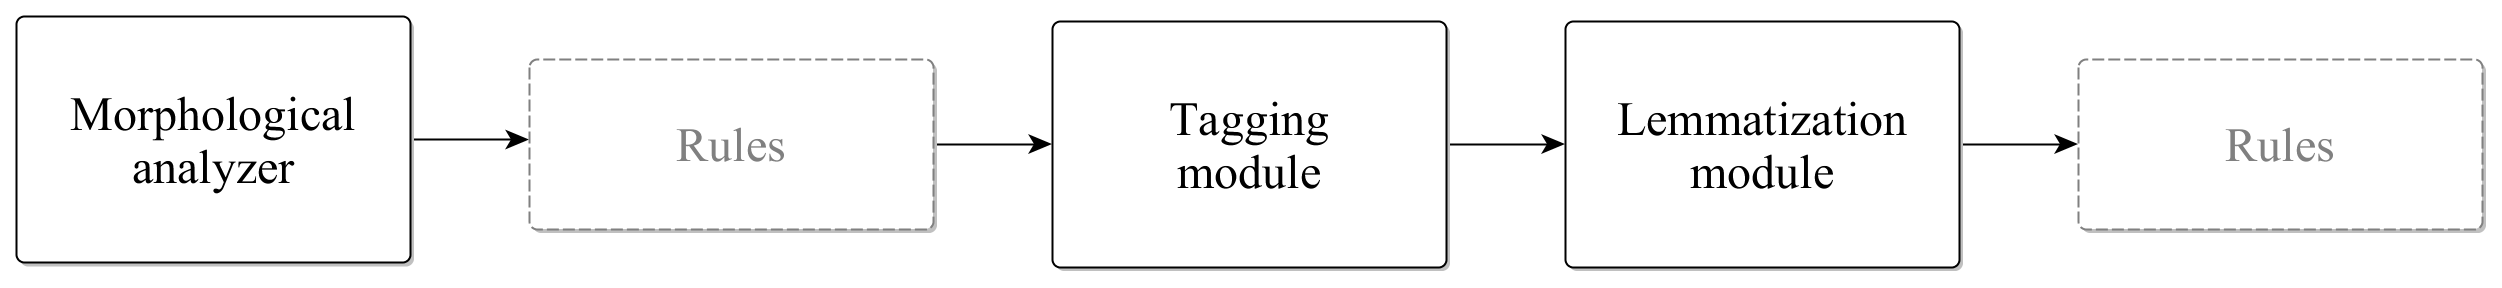
\includegraphics[width=1\textwidth]{MorphTagging/architecture.png} 
  \caption{The architecture of the proposed method}
  \label{fig:purepos-arch}
\end{figure}

In the following, we present its components making the morphological tagging effective. 
In that way,  underlying statistical models are introduced first, then we show how symbolic algorithms are incorporated. 

\subsubsection{The PoS tagging model}

\begin{figure}[H]
  \centering
  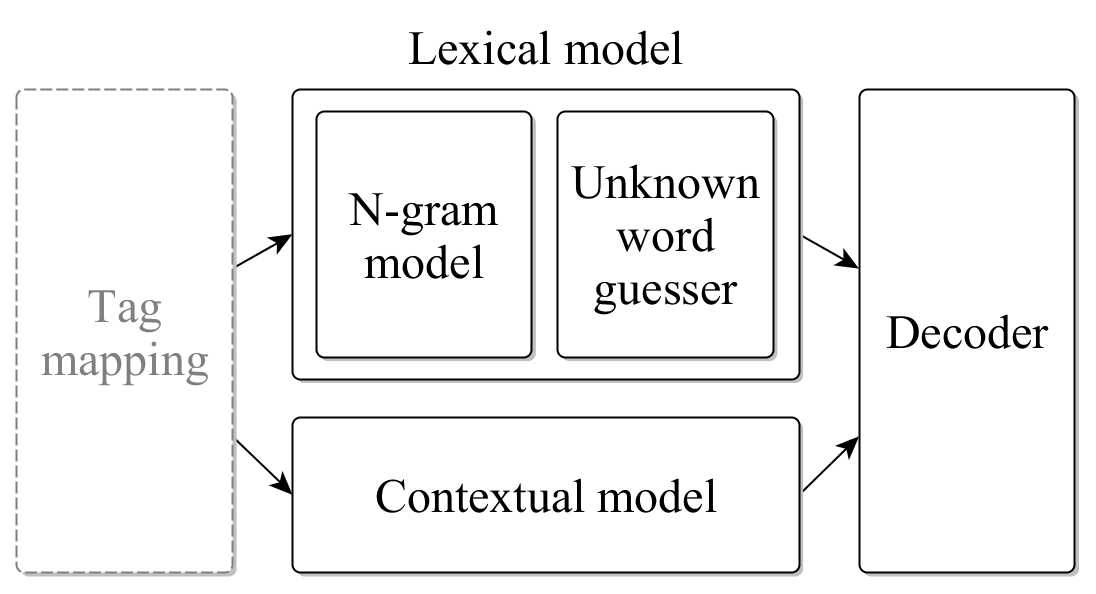
\includegraphics[width=0.5\textwidth]{MorphTagging/pos_arch.png} 
  \caption{Part-of-speech tagging in the proposed system}
  \label{fig:pos_arch}
\end{figure}

PurePos builds on \acrshort{hmm}-based methods \cite{Rabiner1989,Samuelsson1993} introduced in TnT \cite{Brants2000} and HunPos \cite{Halacsy2007}, allowing it to be fast, simple and effective at the same time. 
As its predecessors, our model (see Figure \ref{fig:pos_arch}) selects the best $t_1 \dots t_m$ label sequence for $w_1 \dots w_n$ words by calculating:
\begin{equation}
\argmax_{t_1^m} \prod_{i=1}^m P(t_i | t_{i-1}^{i-n}) P(w_i|t_{i-1}^{i-n})
\end{equation}

Its contextual model is computed with $n$-gram modeling (cf. Equation \ref{eq:purepos-contextual}) employing \gls{mle} (see Equations \ref{eq:purepos-contextual2a} and \ref{eq:purepos-contextual2b})\footnote{Where $N$ denotes the size of the tagset, while $c(x)$ marks the number of $x$ elements in the training data.}. 
Uni-, bi- and trigram estimates are combined with deleted interpolation thus calculating $\lambda_k$ weights as suggested by Brants \cite{Brants2000}. Even though the order of the model is usually set to 3, it is adjustable in practice. 


\begin{equation}\label{eq:purepos-contextual}
P(t_i | t_{i-1}^{i-n}) \approx \sum_{k=0}^{n-1} \lambda_k \hat{P}(t_i|t_{i-1}^{i-k})
\end{equation}

\begin{equation}\label{eq:purepos-contextual2a}
\hat{P}(t_i|t_{i-1}^{i-k}) = \frac{c(t^{i-k}_i)}{c(t_{i-1}^{i-k})} (k>0) 
\end{equation}
\begin{equation}\label{eq:purepos-contextual2b}
\hat{P}(t_i) = \frac{c(t_i)}{N} (k=0)
\end{equation}

Next, the lexical model ($P(w_i|t_{i-1}^{i-n}$) of our method is composed of two components. 
The first one handles tokens previously seen in the training data, while the second guesses labels for unknown words. 
In fact, each subsystem is doubled (as it is in \cite{Brants2000,Halacsy2007}) maintaining separate models for uppercase and lowercase words. 

Handling of previously seen words is carried out approximating $P(w_i | t_{i}^{i-n})$ with word-tag co-occurrences: 
\begin{equation} \label{eq:purepos-lexical}
P(w_i | t_{i}^{i-n}) \approx  \sum_{k=0}^{n-1} \lambda_k \hat{P}(w_i|t_{i}^{i-k})
\end{equation}

\label{sec:purepos-guesser}
$\hat{P}(w_i|t_{i}^{i-k})$ is calculated with \acrlong{mle}, while deleted interpolation is applied with $\lambda_k$ weights. 
As in the contextual model, $k$ is set to 2 in applications.

As regards tagging of unknown words, we use -- in accordance with Brants -- the distribution of rare\footnote{Rare words are considered to be those that occur less than 10 times in the training data.}
tokens’ tags for estimating their \gls{pos} label. 
Since suffixes are strong predictors for tags in agglutinative languages, we use their ($\{s_{n-l+1} \dots s_n\}$) $l$ long combined frequencies:

\begin{align}
 P(t|s_{n-l+1}, \dots, l_n) 
 \approx \frac{ \hat{P}(t|s_{n-l+1}, \dots, s_n) + \theta_i \hat{P}(t|s_{n-l}, \dots, s_n)}{1+\theta_i}
\end{align}

In doing so, $\theta_i$ parameters are calculated applying successive abstraction, while \gls{mle} is utilized  again for computing $\hat{P}(t|s_{n-l+1}, \dots, s_n)$. 

Concerning decoding, beam search is utilized, since it can yield multiple tagging sequences at the same time. 
In that way, the tool is also able to produce tagging scores of sentences \eqref{eq:purepos-score} allowing us to incorporate further components using partly disambiguated word sequences. 

\begin{equation}\label{eq:purepos-score} %%TODO: ez történik, kell ez ide?
Score(w_1^m,t_1^m) = \log \prod_{i=1}^m P(w_i|t_i,t_{i-1})P(t_i|t_{i-1},t_{i-2})P(l_i|t_i,w_i)
\end{equation}

\subsubsection{The lemmatization model}

\begin{figure}[H]
  \centering
  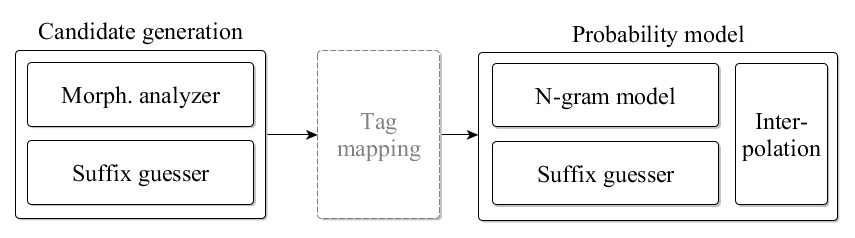
\includegraphics[width=0.8\textwidth]{MorphTagging/lemma_arch.png} 
  \caption{The data flow of the lemmatization component}
  \label{fig:lemma-arch}
\end{figure}

Lemmatization is performed in two steps (cf. Figure \ref{fig:lemma-arch}). 
First, candidates are generated for \emph{(word, morphosyntactic tag)} pairs. 
If morphological analyses are available for the current word, their lemmata are used as candidates, otherwise suffix-based guessing is carried out. 
For this, the guesser (described in Section \ref{sec:purepos-guesser}) was extended to handle lemma transformations as well. 
In doing so, combined labels can represent both the morphosyntactic tag and suffix-transformations for lemmata (for an example see Table \ref{tab:lemma-example}).


\begin{table}[H]
\centering
\caption{Examples for the combined representation of the tag and lemma}
\label{tab:lemma-example}
\begin{tabular}{l | l l}
   \textbf{Word} &  \emph{házam} `my houses’ &  \emph{baglyot} `owl’ \\
   \textbf{Tag} &  \textsc{n.1}s\textsc{pos} &  \textsc{n.acc} \\
   \textbf{Lemma} &  \emph{ház} `house’ &  \emph{bagoly} `owl’ \\
   \textbf{Transformation} & -2+$\varnothing$ &  -4+\emph{oly} \\
   \textbf{Combined label} & (\textsc{n.1}s\textsc{pos}, -2,--) &  (\textsc{n.acc}, -4, \emph{oly}) \\
\end{tabular}
\end{table}


As for picking the right lemma, we utilize a simple scoring model \eqref{lemma-max} that evaluates candidates using their part-of-speech tags:
\begin{equation}\label{lemma-max}
\argmax_l S(l|t,w)
\end{equation}
This method is based on a twofold estimation of $P(l|t,w)$. On the one hand, a unigram lemma model ($P(l)$) calculates conditional probabilities using relative frequency estimates. 
On the other hand, reformulation of $P(l|t,w)$ yields another approximation method:
\begin{equation}\label{lemma-guesser}
P(l|t,w) = \frac{P(l,t|w)}{P(t|w)}
\end{equation}

Substituting this formula to \eqref{lemma-max}, $P(t|w)$ becomes a constant which can be omitted. 
In that way, we can estimate $P(l,t|w)$ employing only the lemma guesser. 
Finally, models are aggregated in a unified ($S$) score: 
\begin{equation}\label{lemma-interpolated}
S(l|w,t) = P(l)^{\lambda_1} P(l,t|w)^{\lambda_2}
\end{equation}


\begin{algorithm*}
\setstretch{1.35}
\begin{algorithmic}[H]
    \ForAll{(word, tag, lemma)} 
        \State candidates $\gets$ generateLemmaCandidates(word, tag)
        \State maxUnigramProb $\gets$ getMaxProb(candidates, word, tag, unigramModel)
        \State maxSuffixProb $\gets$ getMaxProb(candidates, word, tag, suffixModel)
        \State actUnigramProb $\gets$ getProb(word, tag, lemma, unigramModel)
        \State actSuffixProb $\gets$ getProb(word, tag, lemma, suffixModel)
        \State unigramProbDistance $\gets$ maxUnigramProb $-$ actUnigramProb
        \State suffixProbDistance $\gets$ maxSuffixProb $-$ actSuffixProb
        \If {unigramProbDistance $>$ suffixProbDistance}
            \State $\lambda_{2} \gets$ $\lambda_{2}$ $+$ unigramProbDistance $-$ suffixProbDistance
        \Else%If{unigramProbDistance $<$ suffixProbDistance}
            \State $\lambda_{1} \gets$ $\lambda_{1}$ $+$ suffixProbDistance $-$ unigramProbDistance
        \EndIf
    \EndFor
    \State normalize$( \lambda_{1}, \lambda_{2} )$
  \end{algorithmic}
  \caption{Calculating parameters of the lemmatization model}
\label{lemma-interpolation-algorithm}
\end{algorithm*}

The idea of computing $\lambda_{1,2}$ parameters is similar to that seen for the \gls{pos} $n$-gram models. 
However, instead of using positive weights, negative scores are stored for the better model.  
It is calculated iterating over words of the training data (cf. Algorithm \ref{lemma-interpolation-algorithm}):
\begin{enumerate}
  \item first, both components return the best roots for each \emph{(word, tag)} pair, 
  \item then probability estimates for the gold standard lemma are computed,
  \item next, (absolute) error rates of the models are calculated ,
  \item finally, the best model’s weight is decreased\footnote{Since probability estimates are between 0 and 1, decreasing a weight gives higher values.}.
\end{enumerate}
After these steps, $\lambda_k$ parameters are normalized.


\subsubsection{Hybridization}

Although the framework proposed builds on an existing \gls{pos} tagging algorithm, it is extended with a new lemmatization model and is modified to fit agglutinative languages such as Hungarian. 
Hybridization steps listed below show the differences between PurePos and its predecessors \cite{Brants2000,Halacsy2007}.

\begin{description}
  \item[Morphological analyzer] \hfill \\
  First of all, a morphological analyzer is utilized throughout the whole process, therefore probability estimation is performed for valid\footnote{Valid analyses for a word are those which are proposed by the MA.} analyses only.
  \item[Linguistic rules] \hfill \\
  Next, the presented architecture allows rule-based components to modify the analyses of the \acrshort{ma}, in that way, bad candidates can be filtered out. Furthermore, lexical probability scores of analyses can be also given to PurePos, which are then used as context-dependent local distribution functions. 
  \item[Unseen tags] \hfill \\ 
  In contrast to TnT or HunPos, our system is able to handle unseen tags\footnote{Morphosyntactic labels which are not seen in the training data.} properly. On the one hand, if a token has only one analysis not seen before, that one gets selected with 1 lexical probability. Further on, estimation of forthcoming tags are performed using a lower level (unigram) model in this case. On the other hand, the system can also calculate lexical and contextual scores for any tag previously not seen. This can be performed mapping latter tags to a known ones using regular expressions.\footnote{For a complete example see Section \ref{sec:oldhungarian}.}
  \item[$k$-best output] \hfill \\
  Finally, our method decodes tags using beam search. In doing so, one can generate partly disambiguated sentences being apt for linguistic post-processing. Further on, this facility allows the usage of advanced machine learning techniques resulting in more accurate parsing algorithms.
\end{description}


\subsection{Experiments}

\subsubsection{Tagging general Hungarian}\label{sec:porepos-gen}

First, PurePos is evaluated on Hungarian using the Szeged Corpus\footnote{Version 2.3 is utilized in our experiments, since the \acrshort{ma} employed is only compatible with this corpus variation.}~\cite{Csendes2004} (SZC). 
It contains general texts from seven genres being annotated with detailed (MSD) morphosyntactic tags~\cite{Erjavec2012} and lemmata.
Beside the original corpus, we used a variant which is tagged with the analyses of Humor ~\cite{Proszeky1994,Novak2003,Proszeky2005}. 
In our experiments, both corpora were split in 8:2 ratio for training and testing (as in Table \ref{tab:szeged-corpus}) purposes. 

\begin{table}[H]
\centering
\caption{Dimensions of the corpora used}
\begin{tabular}{l r r r r}
  \hline
  & \multicolumn{2}{c}{MSD tagset} & \multicolumn{2}{c}{Humor tagset} \\
  &  Training set &  Test set &  Training set &  Test set  \\
  \hline
  Tokens &  1,232,384 &  254,880 &  980,225 &  214,123 \\
  Sentences &  68,321 &  13,778 &  56,792 &  14,198 \\
  Distinct tags &  1,032 &  716 &  983 &  656 \\
  \hline
\end{tabular}
\label{tab:szeged-corpus}
\end{table}

As a morphological analyzer is an integral part of our method, we tested the tool with two different modules. 
The first setting utilized the MSD tagged corpus and an analyzer extracted from \texttt{magyarlanc}, while the second one applied Humor on the transcribed corpus.

Evaluation is carried out measuring the overall precision of full annotations (i.e \emph{(morphosyntactic tag, lemma)} pairs). 
For significance tests, we have used the Wilcoxon matched-pairs signed-rank test at the 95\% confidence level dividing the test set into 100 data pairs.
Further on, sentence-based accuracies are also provided in some cases. 
The latter metric is computed by considering a sentence to be correct only when all of its tokens are properly tagged. 

Further on, other morphological tagging tools were also evaluated that are available for Hungarian. 
Firstly, \texttt{magyarlanc}, HuLaPos and Morfette\footnote{Version 3.5 is used.} are compared with PurePos.  
%Next, combination of lemmatization and \gls{pos} tagging tools are investigated. 
Secondly, two-phase architectures have been shown to be prosperous (e.g.~\cite{Agic2013,Erjavec2004}), therefore successful modules being commonly applied are also involved in our experiments. 
Concerning \gls{pos} taggers, we use
\begin{itemize}
  \item the trigram tagging method of HunPos,
  \item averaged perceptron learning and
  \item the maximum entropy framework of the OpenNLP~\cite{Baldridge2002} toolkit.
\end{itemize}

As regards lemmatization tools, CST~\cite{Jongejan} and a baseline (as detailed above) method are employed. 
%The latter one results on roots for \emph{(word, tag)} pairs being the most frequent in the training data. 
Beside these components, tag dictionaries have been prepared for HunPos, since it can employ such resources.  
At this point we simulated a setting, where the tagger is only loaded once.
Therefore, a large lexicon was prepared for the tool.
In that way, analyses of the 100,000 most frequent words of Hungarian were provided to the tagger.\footnote{Frequencies are calculated relying on the results of the Szószablya project~\cite{Halacsy2004}.}.

%TODO: keresztvalidáció
%TODO: baseline lemma + purepos

\begin{table}[H]
 \centering
 \caption{Tagging accuracies of Hungarian taggers on the transcribed Szeged Corpus (annotated with MSD labels)}
\begin{tabular}{l r r r}
  \hline
   & \multirow{2}{*}{PoS tagging} & \multicolumn{2}{c}{Morph. tagging} \\
   & &  Token &  Sentence \\
  \hline
  \texttt{magyarlanc} &  96.50\% &  95.72\% &  54.52\% \\
  Morfette &  96.94\% &  92.24\% &  38.18\% \\
  HuLaPos &  96.90\% &   95.61\% & 54.57\% \\
  PurePos &  \underline{96.99\%} &  \underline{96.27\%} &  \underline{58.06\%} \\
  HunPos + BL &  96.71\% &  92.65\% &  36.06\% \\
  HunPos + CST &  96.71\% &  91.19\% &  35.31\% \\
  Maxent + BL &  95.63\% &  92.21\% &  34.82\% \\
  Maxent + CST &  95.63\% &  90.14\% &  29.70\% \\
  Perceptron + BL &  95.19\% &  91.16\% &  29.42\% \\
  Perceptron + CST &  95.19\% &  89.78\% &  27.91\% \\
  \hline
\end{tabular}
\label{tab:morphtag-orig}
\end{table}


\begin{table}[H]
 \centering
 \caption{Tagging accuracies of Hungarian taggers on the transcribed Szeged Corpus (annotated with Humor labels)}
\begin{tabular}{l r r r}
  \hline
   & \multirow{2}{*}{PoS tagging} & \multicolumn{2}{c}{Morph. tagging} \\
   & &  Token &  Sentence \\
  \hline
  Morfette &  97.60\% &  94.73\% &  51.58\% \\
  HuLaPos &  97.19\% &  95.53\% &   57.55\% \\
  PurePos &  \underline{98.65\%} &  \underline{98.58\%} &  \underline{81.78\%} \\
  HunPos + BL &  97.41\% &  89.93\% &  32.07\% \\
  HunPos + CST &  97.41\% &  94.69\% &  52.40\% \\
  Maxent + BL &  94.81\% &  88.82\% &  28.19\% \\
  Maxent + CST &  94.81\% &  92.33\% &  40.10\% \\
  Perceptron + BL &  95.97\% &  88.85\% &  29.11\% \\
  Perceptron + CST &  95.97\% &  93.32\% &  45.13\% \\
  \hline
\end{tabular}
\label{tab:morphtag-humor}
\end{table}

% % % % % % % % % % % % % % % % % % % % % % % % % % % % % % % % % % % %
First of all, there are notable discrepancies between the results on the two datasets (cf. Tables \ref{tab:morphtag-orig} and \ref{tab:morphtag-humor}). 
On the one hand, performance discrepancies can be explained by the morphological analyzers used.
These tools have different coverage, thus they affect the results of parsing chains built on them.
On the other hand, the two corpora utilize different annotation schemes:
\begin{itemize}
  \item First, the original corpus contains foreign and misspelled words being tagged with a uniform \textsc{x} tag. 
  Due to the various syntactic behavior of such tokens, their labels could not be estimated using their context or their suffix properly.
  \item Further on, date expressions and several named entities are tagged with a single MSD code resulting in lemmata composed of more than one words. (An example is \emph{Golden Eye-oztunk} `we visited the Golden Eye’ being lemmatized as \emph{Golden Eye-ozik} `to visit the Golden Eye’.) 
  Such phenomena could be hard to handle for lemmatizers.
\end{itemize}
These differences can have a huge impact on morphological disambiguation algorithms.
In our case, they decrease the accuracy of MSD-based systems, while allow Humor-based ones to produce better annotation  (since the corresponding corpus is free of such phenomena).

In general, results show that the best-performing systems are PurePos, HuLapos, \texttt{magyarlanc} and Morfette.
Besides, HunPos also achieves high \acrshort{pos} tagging scores, while other two-stage taggers are far behind state-of-the-art results. 
As regards learning methods of the OpenNLP toolkit, their precision indicate that they cannot handle such labeling problems precisely.
Further on, both of the standalone lemmatizer degrade accuracy. 
This reduced performance can be due to their design: the baseline method was not prepared for handling unknown words, while CST was originally created for inflectional languages. 

An explanation for the high morphosyntactic labeling score of PurePos is that it uses morphological analyzers to get analyses candidates. 
This component can reduce the number of unknown words, thus enabling it to provide better annotations.
While HunPos also uses such resources, it can only handle static lexicons which limits its accuracy.
%In that way, the huge number of inflected word-forms could be handled accurately.

As regards \texttt{magyarlanc}, it also yields first-class results (95.72\% precision) on the MSD-tagged corpus, however, its language specific components inhibit its application on other corpora. 
Further on, HuLaPos is an interesting outlier.
It is based on pure stochastic methods, but it can still achieve high precision.
Next, Morfette also provides accurate annotations (concerning \acrshort{pos} labels only), however it has problems with computing the roots of words.

Results show that PurePos provides the most accurate annotations amongst tested tools.
Further on, its advance over other systems is statistically significant (Wilcoxon test of paired samples, p < 0.05)\footnote{Pairwise tests were carried out comparing token-level accuracies of PurePos and other competing tools on each corpus.}.
In addition, sentence-based accuracies (especially on the Humor-tagged corpus) also confirms the superior performance of our method. 
These values reveal that most of the tools result in erroneously tagged sentences in more than half of the cases, while the same number for our method is much less (42\% and 18\% respectively). 

It was shown that the presented algorithm can produce high quality morphosyntactic annotations handling the huge number of inflected forms of Hungarian.
Further on, it can also produce precise root candidates for both previously seen and unseen tokens due to its improved lemma computing method.
In that way, Purepos is a suitable tool for morphological tagging of Hungarian and other agglutinative languages.
%
%Next, comparison of full annotation scores reveals that our lemmatization algorithm significantly outperforms others. 
%Furthermore, its lemmatization method outperforms all other systems available for Hungarian.

\subsubsection{Resource-scarce settings}

Next, PurePos is compared to other taggers on less-resourced scenarios.
For this we use systems\footnote{Unfortunately, we could not measure the performance of \texttt{magyarlanc}, since the current release of the tool cannot be trained.})  and corpora described in Section \ref{sec:porepos-gen}.
For this, the amount of the training data was limited (cf. Table \ref{tab:small-szeged}).
In that way, we draw learning curves of systems, evaluating them on both versions of the test set.

\begin{table}[H]
\centering
\caption{The number of tokens and sentences used for training the taggers}
\label{tab:small-szeged}
\begin{tabular}{ r | r r r r r}
Sentences & 2,000 & 4,000 & 6,000 & 8,000 & 10,000 \\
Tokens (MSD-tagged corpus) & 13,555 & 26,496 & 53,563 & 79,916 & 107,113 \\
Tokens (Humor-tagged corpus) & 20,863 & 41,740 & 82, 964 & 121,026 & 146,816 \\
\end{tabular}
\end{table}


\begin{figure}[H]
  \centering
  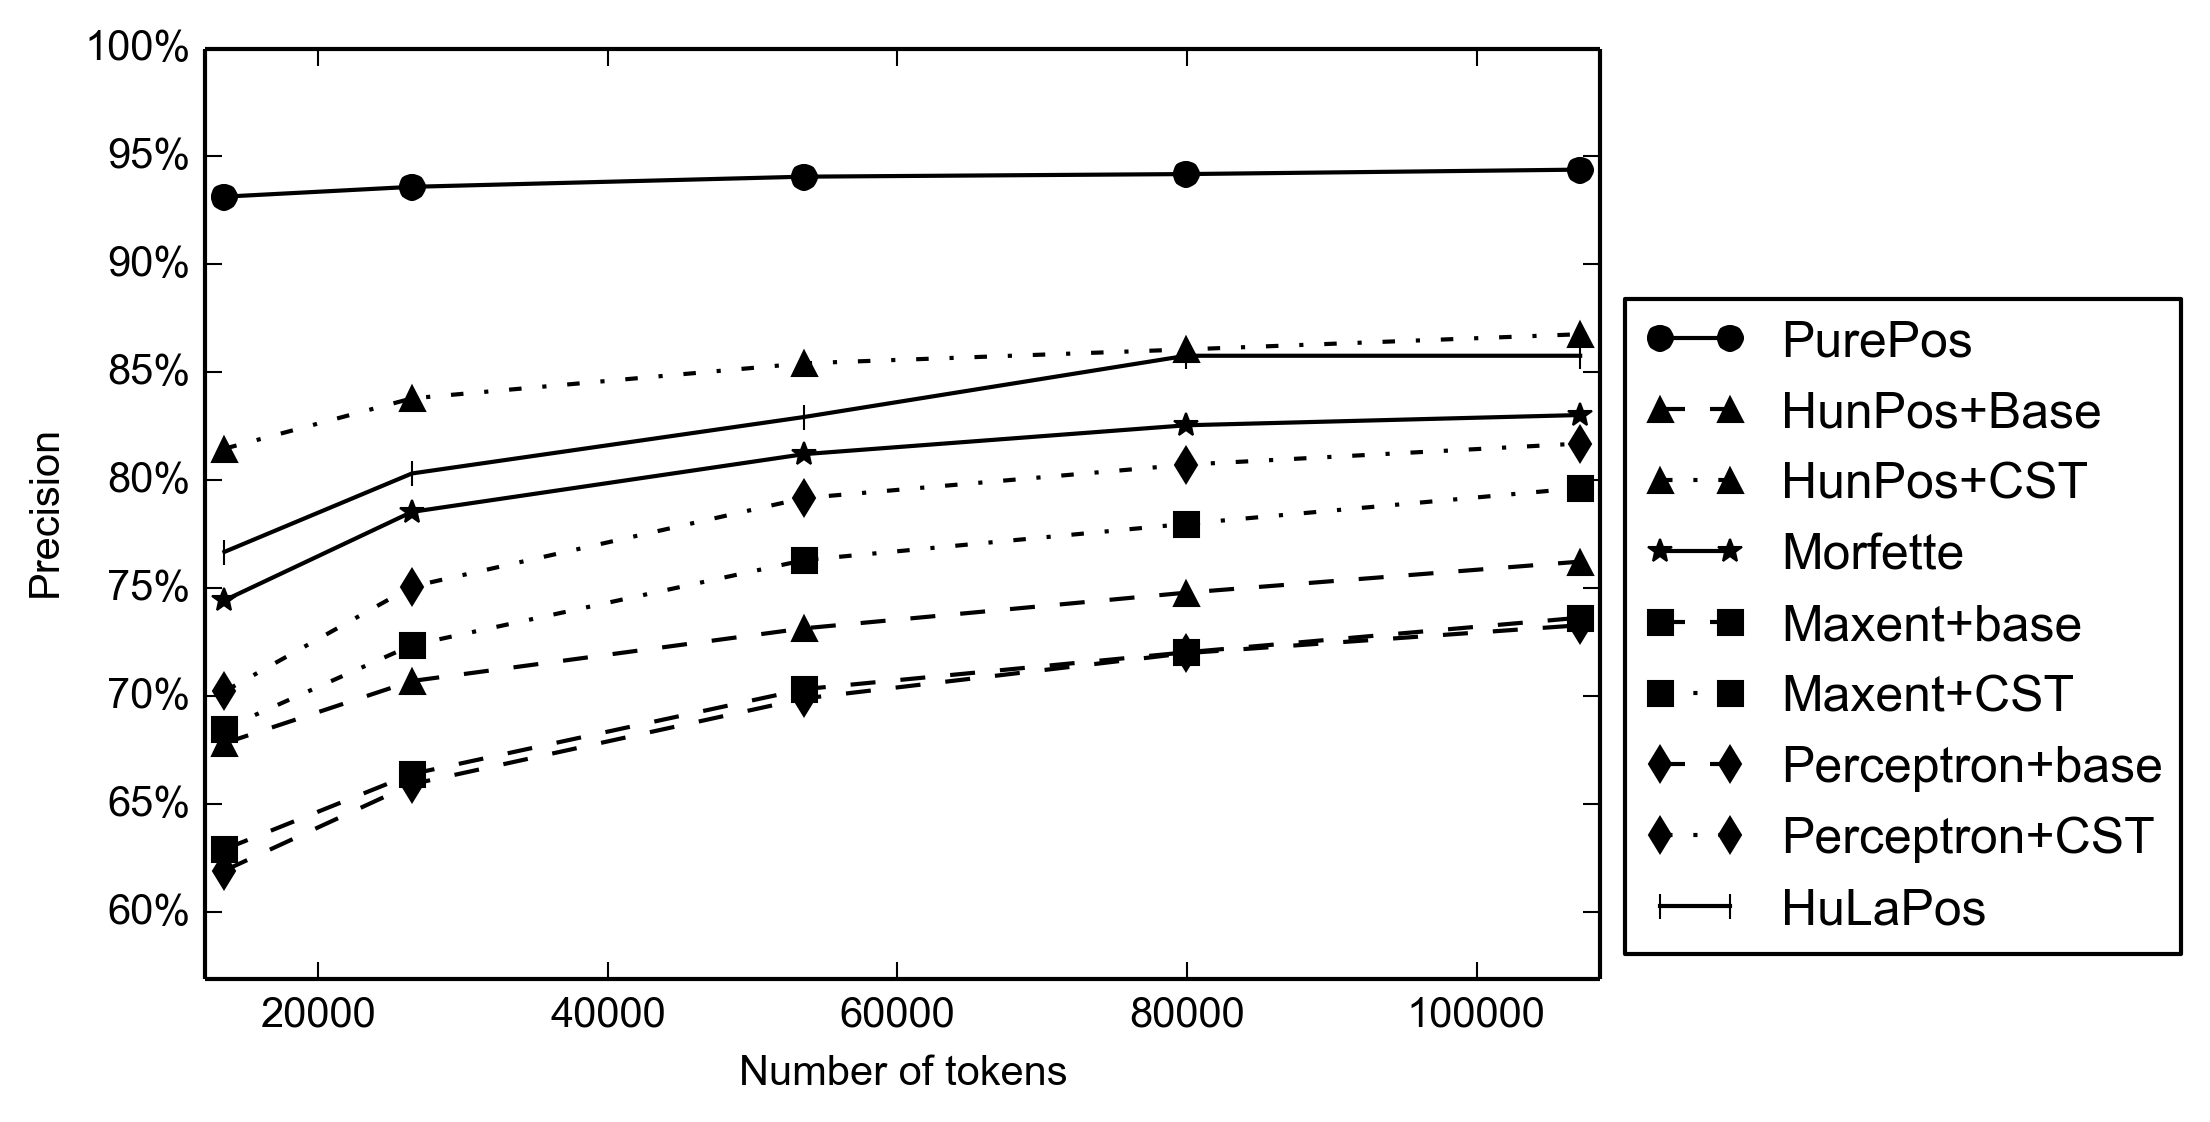
\includegraphics[width=1\textwidth]{MorphTagging/msd_token.png} 
  \caption{Learning curves (regarding token accuracy) of full morphological taggers on the Szeged Corpus (using MSD labels)}
  \label{fig:msd-token}
\end{figure}

\begin{figure}[H]
  \centering
  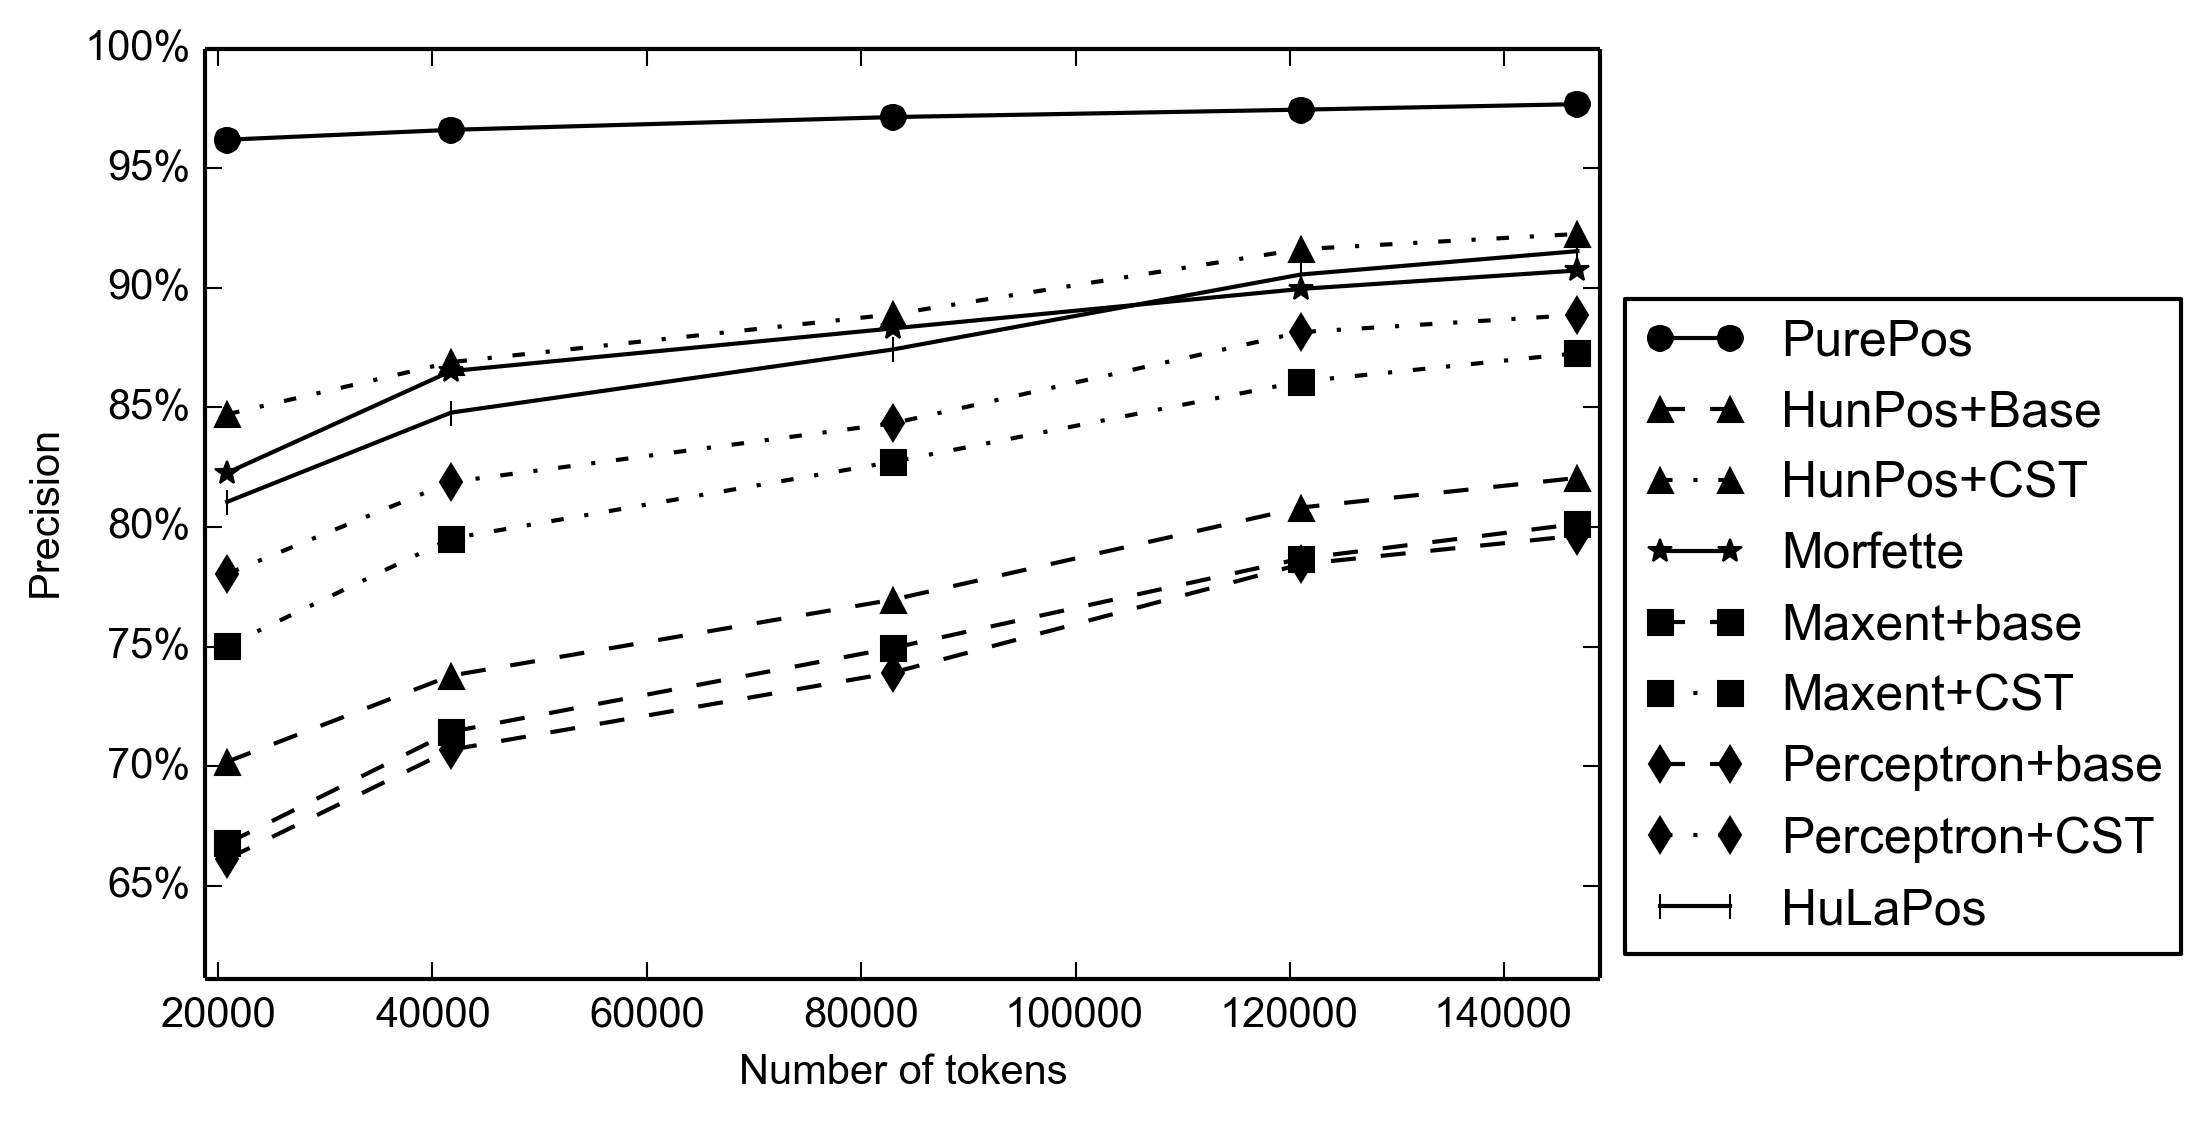
\includegraphics[width=1\textwidth]{MorphTagging/humor_token.png}
  \caption{Learning curves (regarding token accuracy) of full morphological taggers on the Szeged Corpus (using Humor labels)}
  \label{fig:humor-token}
\end{figure}

\begin{figure}[H]
  \centering
  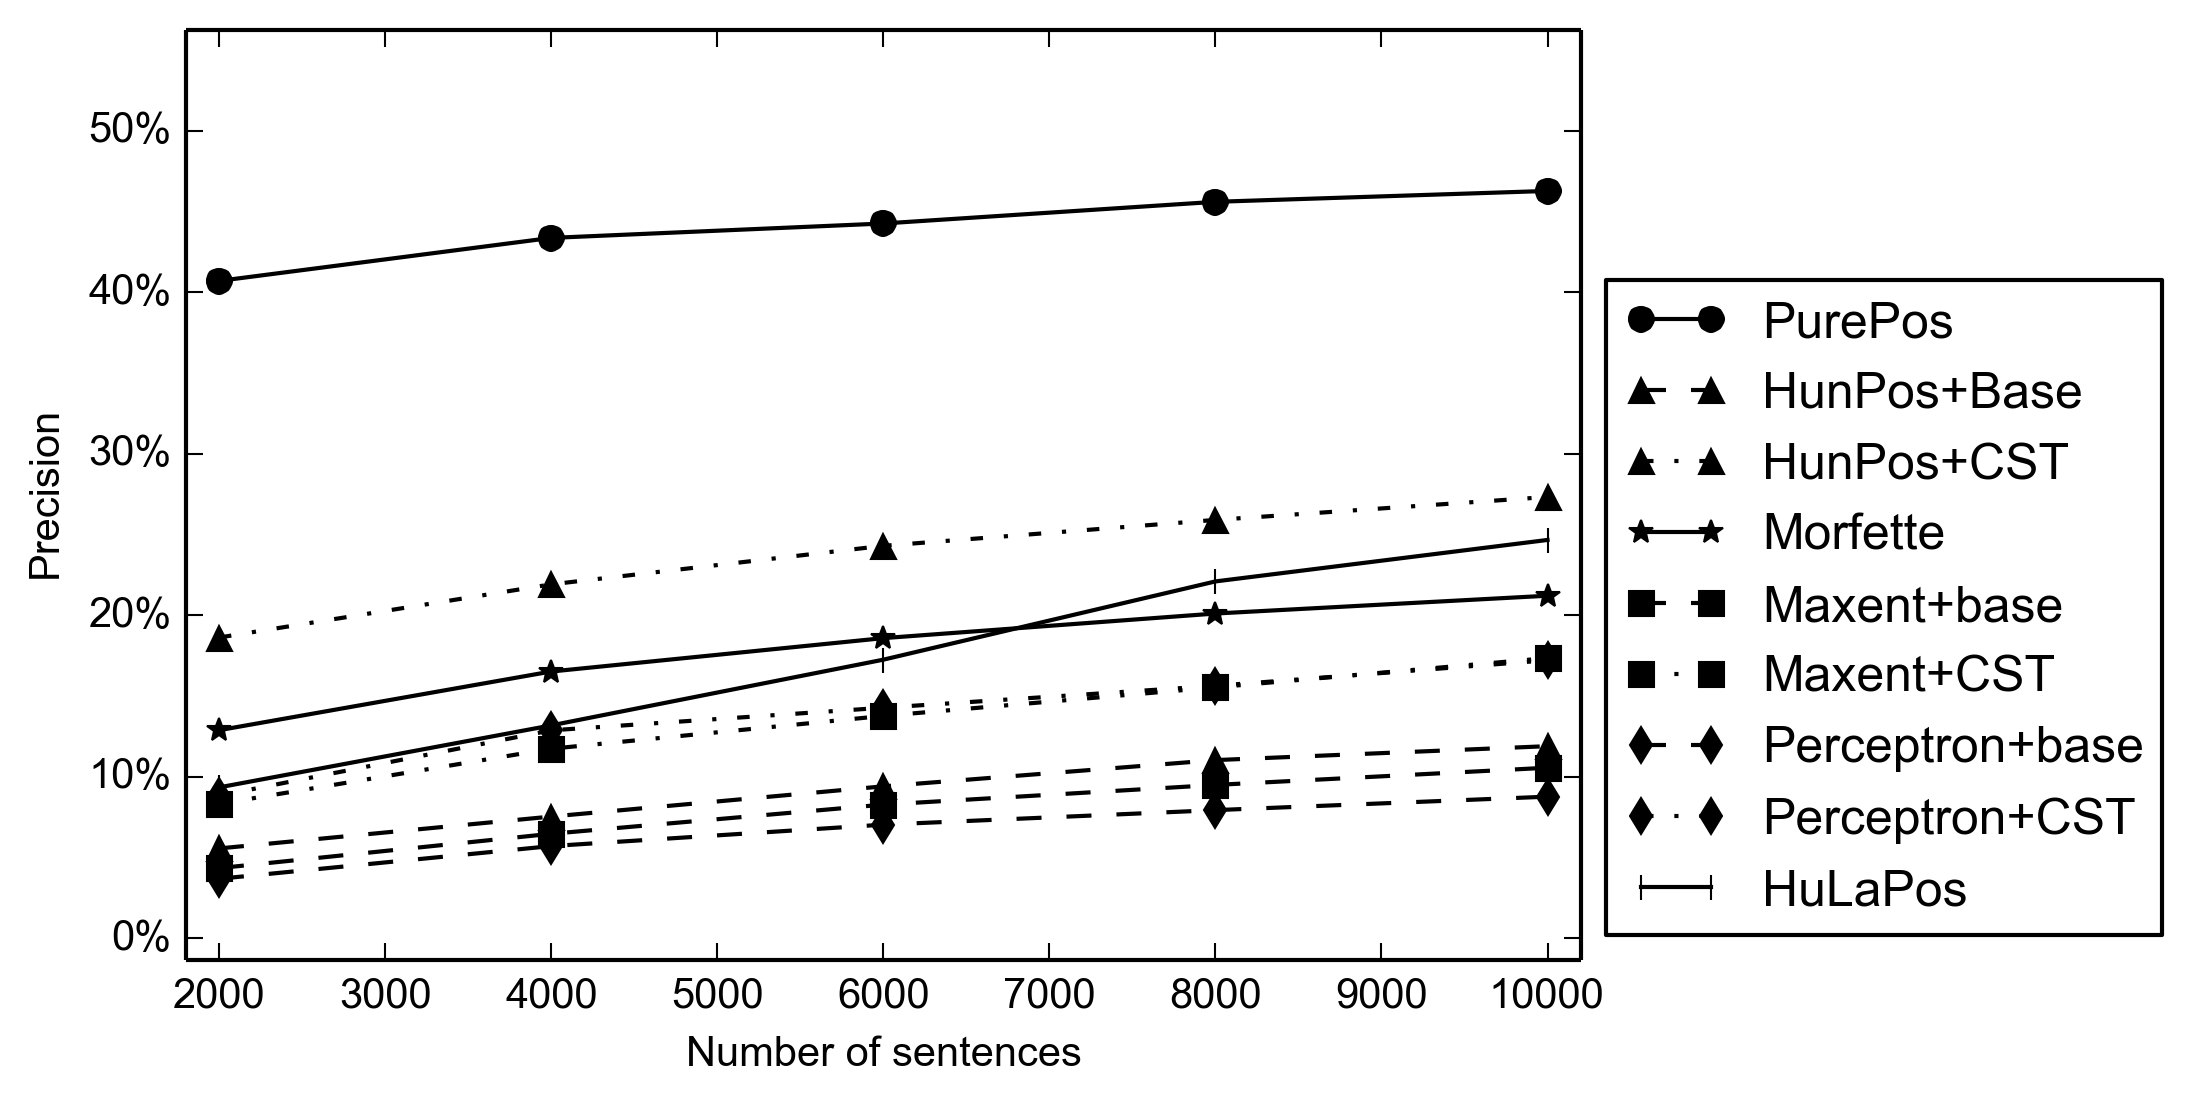
\includegraphics[width=1\textwidth]{MorphTagging/msd_sent.png} 
  \caption{Learning curves (regarding sentence accuracy) of full morphological taggers on the Szeged Corpus (using MSD labels)}
  \label{fig:msd-sent}
\end{figure}

\begin{figure}[H]
  \centering
  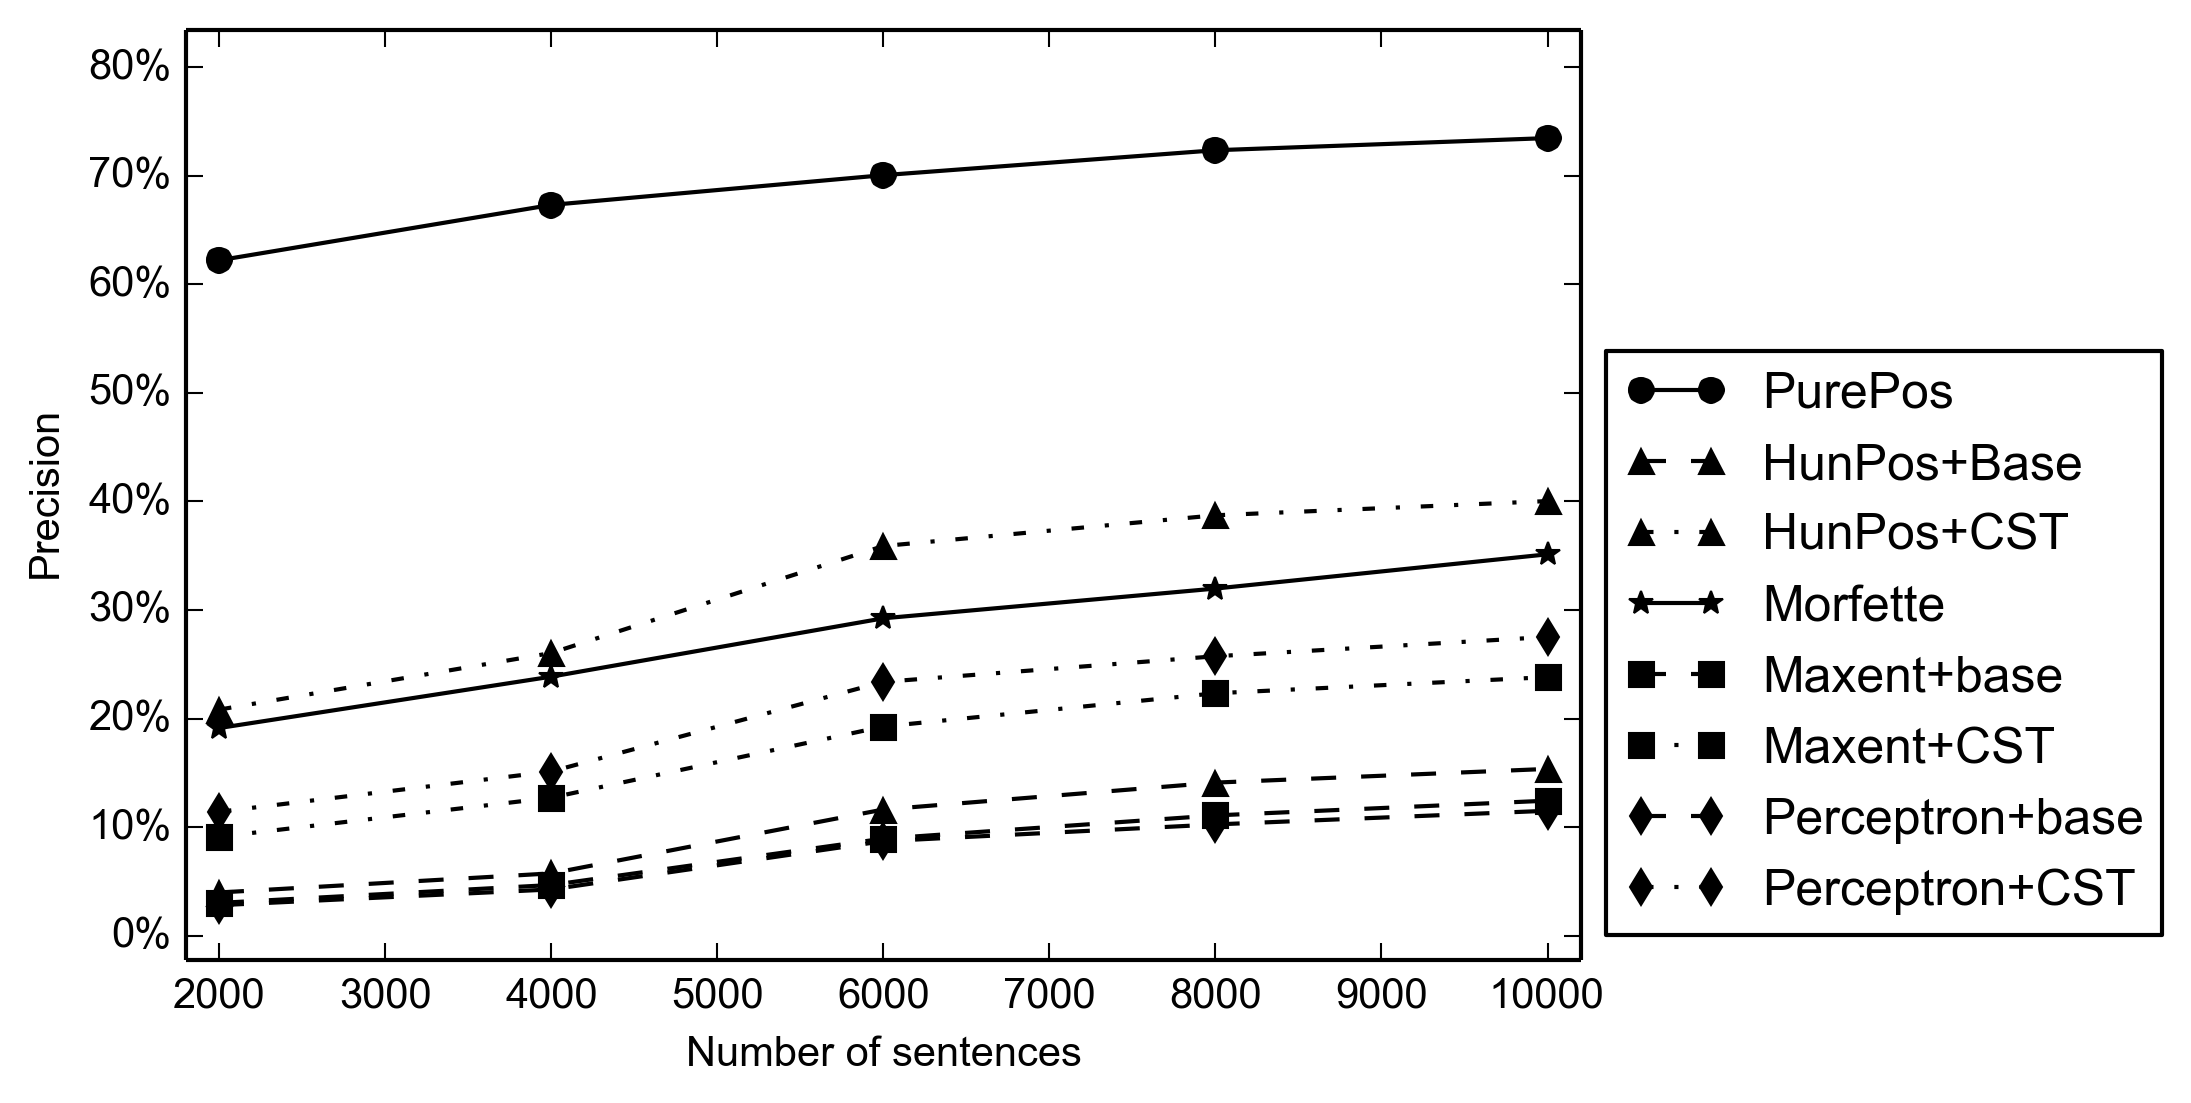
\includegraphics[width=1\textwidth]{MorphTagging/humor_sent.png}
  \caption{Learning curves (regarding sentence accuracy) of full morphological taggers on the Szeged Corpus (using Humor labels)}
  \label{fig:humor-sent}
\end{figure}

First, Figures \ref{fig:msd-token} and \ref{fig:humor-token} present morphological tagging accuracies of systems depending on the number of tokens in the training corpus. 
These results are in accordance with conclusions of our previous experiments, however the differences revealed are higher. 
Further on, the large distance between the precision scores of PurePos and other tools confirms the effectiveness of our  hybrid approach in less-resourced scenarios.


Further on, if we compare (cf. Figures \ref{fig:msd-sent} and \ref{fig:humor-sent}) the taggers' sentence-based precisions, the gap between their performance are much more emphasized. 
For example, having only 2,000 sentences for training (with MSD tags) the proposed algorithm results in 40.71\% sentence precision compared to the second best of 18.62\%.

In brief, we have shown that the architecture of PurePos allows producing accurate annotations when the amount of training data is limited. Therefore, our method could be used for morphological tagging scenarios of agglutinative languages when there is just a few thousand manually annotated sentences are available.

\subsubsection{The case of Middle- Old-Hungarian}
\label{sec:oldhungarian}

Next, we present a tagging task showing the effectiveness of all the hybrid components available in PurePos. 
In a project~\cite{NovakOMK,Novak2013} aiming at the creation of an annotated corpus of Middle Hungarian texts, an adapted version of the Hungarian Humor morphological analyzer \cite{NovakOMK} was used\footnote{The adaptation of Humor and the annotation are the work of Attila Novák and Nóra Wenszky. The author's contribution is the enhancement of the morphological tagging chain.}. 
This tool was originally made to annotate contemporary Hungarian, but the grammar and lexicon were modified to handle morphological constructions existed in Middle Hungarian but have since disappeared from the language. 
In the experiments described here, we used a manually disambiguated portion of this corpus. The data was labeled using a rich variant of the Humor tagset having cardinality over a thousand.

\begin{table}[H]
\centering
\caption{Characteristics of the used corpus}\label{tab:oldhun-corpus}
\begin{tabular}{l r r r}
\hline
& Training & Dev. & Test \\
\hline
Documents & 140 & 20 & 30 \\
Clauses & 12,355 & 2,731 & 2,484 \\
Tokens & 59,926 & 12,656 &  11,763\\
\hline
\end{tabular}
\end{table}

The corpus is split into three parts (see Table \ref{tab:oldhun-corpus}) for the experiments. 
The tagger was trained on the biggest one, adaptation methods were developed on a separate development subcorpus, while final evaluation was done on the test set.
We used precision as an evaluation metric, but unambiguous punctuation tokens were \emph{not} taken into account (in contrast to how taggers are evaluated in general). 
They are ignored because the corpus contains a relatively large amount of punctuation markers which would distort the comparison.
Methods were evaluated twofold: full morphological disambiguation accuracies were calculated for tokens and they were also computed to obtain clause-level precision values. 
In addition, \gls{err} \eqref{eq:err} is calculated measuring the percentage of mistakes ($E$) of a baseline tagger ($b$) that are corrected by an enhanced method ($n$). 

\begin{equation}\label{eq:err}
\err(b,n) = \frac{E(b)-E(n)}{E(b)}
\end{equation}

We used the improved trigram-based algorithm derived from HunPos and implemented in PurePos (PP) as a baseline \gls{pos} tagger. 
This basic chain is enhanced step-by-step investigating the impact of each component.
First, the \acrshort{ma} and the new lemmatization method is analyzed on the development set (cf. Table \ref{tab:oldhun-baselines}). 

\begin{table}[H]
\centering
\caption{Baseline disambiguation accuracies on the development set}\label{tab:oldhun-baselines}
\begin{tabular}{l r r r}
\hline
 & Tokens & Clauses \\
\hline
% PP+BL & 93.20\% & 88.99\% & 55.58\% \\
PP+BL  & 88.99\% & 55.58\% \\
% PP+SL & 93.20\% & 89.01\% & 51.78\% \\
% PPM+BL & 97.77\% & 97.22\% & 84.85\% \\
PPM+BL  & 97.22\% & 84.85\% \\
% PPM+SL & 97.77\% & 97.50\% & 85.98\% \\
PP + CL & 92.14\% & 65.40\% \\
PPM + CL & 97.58\% & 86.48\% \\
\hline
\end{tabular}
\end{table}


On the one hand, we compare the \gls{pos} tagging method of PurePos with (PPM) and without the morphological analyzer (PP).
On the other hand the simple unigram-based (BL) lemmatizer (cf. Section \ref{sec:purepos-guesser}) is evaluated against the proposed one (CL). 
First, it was found that the usage of a morphological component is indispensable. 
Next, results show that the proposed algorithm yields a significant error rate reduction compared to the baseline. 
This improvement is even more notable  (28.42\% \acrshort{err}) when a dedicated morphological analyzer is not used.

In the next, several experiments are presented to exhaust hybrid facilities of PurePos, thus yielding a more accurate tagger. 
To that end, the development set was utilized to analyze common error types and to develop hypotheses.

\paragraph{Mapping of tags}

In contrast to other Hungarian annotation projects, the tagset of the historical corpus distinguishes verb forms that have a verbal prefix from those that do not, because this is a distinction important for researchers interested in syntax.\footnote{Hungarian verbal prefixes or particles behave similarly to separable verbal prefixes in most Germanic languages: they usually form a single orthographic word with the verb they modify, however, they are separated in certain syntactic constructions.} 
This practically doubles the number of verb tags\footnote{320 different verb tags occur in the corpus excluding verb prefix vs. no verb prefix distinction. This is just a fraction of the theoretically possible tags.}, which results in data sparseness problems for the tagger. 
In the case of a never encountered label having a verbal prefix marking, one can calculate probability estimates for that tag by mapping it to one without a verbal prefix. 
This solution is viable, since the distribution of prefixed and non-prefixed verbs largely overlap. 
Applying this enhancement (TM), we could increase notably the accuracy of the system on the development set (to 86.53\% clause level precision).

\paragraph{Preprocessing}

Another point of improvement is to filter analyses of Humor (FI). 
Exploiting the development set, a preprocessing script was set up which has five simple rules. 
Three of them catches the tagging of frequent phrases such as \emph{az a} `that' in which \emph{az} must be a pronoun. 
Further on, two domain specific lexicons were employed to correct the erroneous annotation of proper names that coincide with frequent common nouns or adjectives. 
Using these correction rules the overall performance on the development set was further raised to 86.77\% clause accuracy.


%%%%%%%%%%%%%%%%%%%%%%%%%%%%%%%%%%%%%%%%%%%%%%%%%%%%%%%%%%%%%%%%%%%%

\paragraph{$k$-best output}
The $k$-best output of the tagger can either be used as a representation to apply upstream grammatical filters to or as candidates for alternative input to higher levels of processing. 
Five-best output for our test corpus has yielded an upper limit for attainable clause accuracy of 94.32\% (on the development set). 
%These can either be used as a representation to apply upstream grammatical filters to or as candidates for alternative input to higher levels of processing.
While it is not directly comparable with the ones above, this feature could e.g. be used by syntactic parsers.


\begin{table}[H]
\centering
\caption{Disambiguation accuracies of the hybrid tool on the test set}
\label{tab:oldhun-test}
\begin{tabular}{l r r r}
\hline
 & Full & Clauses  \\
\hline
Baseline  & 89.47\% & 55.07\% \\
PurePos  & 96.48\% & 80.95\% \\
\hspace{0.2cm} + TM  & 96.51\% & 81.17\% \\
\hspace{0.2cm} + FI  & 96.60\% & 81.55\% \\
\hspace{0.2cm} + all  & 96.63\% & 81.77\% \\
\hspace{0.2cm} + all with \emph{k}-best  & 98.66\% & 92.30\% \\
\hline
\end{tabular}
\end{table}
 
Enhancements are validated evaluating them on the test set.
Data in Table \ref{tab:oldhun-test} shows that each linguistic component improves the overall chain significantly\footnote{We used the Wilcoxon matched-pairs signed-rank test at p < 0.05}.
Further on, using the $5$-best output sequence of the tagger provides us much more golden annotations. 
These are available for 92.30\% of the clauses and for 98.66\% of the tokens.

Therefore, we have shown that one can further increase the tagging accuracy by employing hybrid facilities of PurePos. 
%In this section, linguistic knowledge has been used to raise the overall accuracy.
First, rules were employed filtering our erroneous analyses candidates, then unseen tags were mapped to previously seen ones successfully. 
Finally, we have shown that the 5-best output contain significantly more golden annotations.





% \pagebreak

\section{Combination of morphological taggers}\label{sec:combination}
Although high accuracy tagging tools are generally available, sometimes their performance is not satisfactory and shall be increased further.
In cases where very high annotation quality is required, variance of tools should be considered.
Disparate methods can result in different sorts of errors, therefore their combination can yield better algorithms.
Even though this idea is not new, being present in both machine learning and \acrshort{nlp} literature, there has not been much work done on in this field for morphologically rich languages. 

In this section, the case of agglutinative languages is investigated by experimenting with Hungarian morphological disambiguator tools.
First, we give a brief overview about \acrshort{pos} tagger combination methods.
Next, discrepancies of two taggers are presented allowing us to create a new combination architecture.
Finally, we evaluate the proposed method by measuring its improvement over baseline tools used.

\subsection{Background}

The design process of a combined tagger system involves several steps\footnote{Statements are based on studies of Brill and Wu~\cite{Brill1998} and Halteren et al.~\cite{Halteren2001}.}.
First, it needs to be examined whether the errors of components are different enough to outperform the best individual system significantly.
Then an appropriate combining scheme must be found.
Decisions to be made by a combination algorithm can be of at least two sorts: 
\begin{enumerate}
  \item it can either always select the output of one of the bottom-level systems, or 
  \item it can generate an output of its own that may differ from the output of each individual embedded system. 
\end{enumerate}

When applying the former solution, errors of embedded systems determine a theoretical upper limit on the accuracy of the combined system, since it can never generate the expected output whenever neither of the embedded classifiers generate it.
Thus, the latter solution seems more beneficial in theory.
However, the complexity of the annotation task to be performed and the available training data may have an influence on which of these options is feasible and how they perform in practice.
E.g. if the cardinality of the output annotation and features involved in training is high, there may be either data sparseness or performance problems with the second option.

As regards combination strategies, a basic method is majority voting.
Other, more advanced, schemes involve training a top-level classifier based on the individual embedded systems.
This class of schemes is commonly referred to as stacking learners.
The top-level classifier may use various features of both the inputs and the outputs of the bottom-level classifiers when making its decision. 

One of the first attempts of combining English PoS taggers was presented by Brill and Wu \cite{Brill1998}.
They propose memory-based learning which employs contextual and lexical clues.
In their experiments, the solution where the top-level learner always selects the output of one of the embedded taggers outperformed the more general scheme that allowed the output differ from either of the proposed tags.
Next, a comprehensive study by van Halteren et al. \cite{Halteren2001} details an overview of previous combination attempts.
Further on, the authors show that cross-validation can be used to train top-level classifiers for an optimal utilization of the corpus.
They found a scheme performing best characterized as generalized voting.
Although it can yield annotation differing from the output of the embedded taggers, it can also be interpreted as a stacking method.
However, the cardinality of the tag set and the dimensionality of the feature space were modest compared to that of our case.

A system of different architecture is presented by Hajič et al. \cite{Hajic2001}: in contrast to the parallel and hierarchical architecture of the systems above, it employs a serial combination of annotators starting with a rule-based morphological analyzer, followed by constraint-based filters feeding statistical taggers at the end of the chain. 

We use metalearners with cross-validation, since such schemes \cite{Brill1998,Halteren2001} perform effectively.
Further on, language-specific symbolic components are utilized as well, as they can help to handle the rich morphology of the target language.
%In that way, we improve existing methods. 
First, the underlying architecture of general combination methods is modified to produce lemmata candidates as well.
Then, features investigated which fit the best for agglutinative languages.

\subsection{Discrepancies of taggers}

Evaluating taggers on general Hungarian can show that two of the best performing tools (our new method and HuLaPos) significantly diverge by the errors they made.
In our evaluation scheme, a detailed analysis of errors was carried out first, aiming to reveal their possible combined performance.
For this, we utilized the Humor-tagged Szeged Corpus (described in \ref{sec:porepos-gen}).
We kept the training sentences (80\% of the corpus), but the rest was split into two parts. The first half was employed for development purposes, while the second one was set apart for the final evaluation (cf. Table \ref{tab:comb-data}).

\begin{table}[H]
\centering
\caption{Number of sentences and tokens used for training, tuning and evaluating combination algorithms}\label{tab:comb-data}
\begin{tabular}{l r r}
\hline
& Tokens & Sentences \\
\hline
Training set & 980,225 & 56,792\\
Development set & 105,779 & 7,099 \\
Test set & 108,344 & 7,099 \\
\hline
\end{tabular}
\end{table}

First of all, we could not compare word class error rates one-by-one to reveal differences of taggers, since the cardinality of the tagset is over 1,000.
Further on, we could neither rely on Brill's well-known formula (cf. \cite{Brill1998}), as it gives hard-to-interpret unlimited negative values when there is a considerable amount of overlap between the errors investigated.
Therefore, a new metric, called Own Error Rate ($\oer$), was introduced to measure the relatedness of the taggers' errors.
We used the formula 
\begin{equation}
\oer(A,B)=\frac{\text{\#errors of }A\text{ only}}{\text{\#errors of either }A\text{ or }B}
\end{equation}
for calculating the percentage of tagger $A$ being wrong but $B$ being correct in proportion of all errors made by either $A$ or $B$.

\begin{table}[H]
\centering
\caption{Error analysis of PurePos and HuLaPos on the development set}\label{tab:comb-disambig-comp}
\begin{tabular}{l r r r}
\hline
& Tagging & Lemmatization & Full disambig. \\
\hline
% \hline
% Disagreement rate& 2.40\% & 1.98\% & 3.08\% \\
Agreement rate & 97.60\% & 98.02\% & 96.92\% \\
%Agr on not correct/One mistags & 22.09\% & 7.10\% & 18.26\% \\
They are right when they agree & 99.30\% & 99.85\% & 99.29\% \\
%%Agreement on erroneous annotation & 0.70\% & 0.15\% & 0.61\% \\
One is right when they disagree & 97.53\% & 98.89\% & 97.14\% \\
%\hline
$\oer($PP, HL$)$ & 22.41\% & 11.66\% & 21.16\% \\
$\oer($HLP, PP$)$ & 53.58\% & 80.21\% & 58.24\% \\
\hline
\end{tabular}
\end{table}

To begin, we investigated the agreement of tools on the development set.
As Table \ref{tab:comb-disambig-comp} shows:
\begin{enumerate}
 \item they agree on the full annotation in most of the cases,
 \item matching tags and lemmata are almost always right, 
 \item one of them (frequently) knows the correct annotation even when their guesses do not match.
\end{enumerate}

Secondly, own error rates indicate that even though HuLaPos performs worse than PurePos, the errors are fairly balanced between them. 

\begin{table}[H]
\centering
\caption{Precision of the oracle and baseline systems on the development set}\label{tab:comb-disambig-acc}
\begin{tabular}{l r r r}
\hline
& Tagging & Lemmatization & Full disambig. \\
\hline
PurePos & 98.57\% & 99.58\% & 98.43\% \\
HuLaPos & 97.61\% & 98.11\% & 97.03\% \\
Oracle & 99.26\% & 99.83\% & 99.22\% \\
\hline
\end{tabular}
\end{table}

Finally, the theoretical maximum performance of the combination (marked as oracle) is presented in Table \ref{tab:comb-disambig-acc}.
Assuming a hypothetical oracle always selecting the correct \emph{(tag, lemma)} pairs from the tools' suggestions, the accuracy of the better tagger can be further increased eliminating 72.73\% of PurePos' errors. 

\subsection{Improving PurePos with HuLaPos}

To utilize combination through cross-validation, the training set was split into 5 equal-sized parts.
Level-0 taggers (PurePos and HuLaPos) were trained 5 times using the 4/5 of the corpus while the rest of the sentences were annotated by both taggers in each round.
The union of these automatically annotated parts were used to train the (level-1) metalearners.
Furthermore, this technique allowed us to utilize all the training data in each level, yet separating the two phases of the training process. 

Concerning the question of choosing a level-1 learner we followed Witten et al. \cite{Witten2011} for investigating only ``relatively global, smooth'' algorithms.
We utilized \footnote{C4.5 decision tree algorithm was involved in our experiments, but it was unable to handle the large amount of feature data used.} the naïve Bayes (NB) classifier \cite{John1995} and instance-based (IB) learners \cite{Aha1991}.
The latter in addition to be simple, had been previously shown to perform well in similar combination tasks.
Another important decision was to apply metalearners only in cases of disagreement, since the tools’ agreement rate was high.

There are at least two parameters which must be set for IB learners.
First, a distance function needs to be selected, then the number of neighborhooding events has to be restricted.
In that way, we opted on using Manhattan distance and decided to rely only on the single closest item. 

Moving on, Hungarian has a tagset with a cardinality of over a thousand and an almost unlimited vocabulary, which would make the tag-picking approach inviable. Therefore, we applied methods choosing the tagger but not the tag. 

As regards features, we relied on the set proposed by Brill and Wu \cite{Brill1998}, since it had been shown (cf. \cite{Halteren2001}) to be simple but powerful. It (FS1 in Table \ref{tab:comb-feature-sets}) consists of several lexical properties such as
\begin{enumerate}
 \item the word to be tagged, 
 \item immediate neighbours of the token,
 \item tags suggested for the corresponding word,
 \item tags suggested for neighbouring tokens.
\end{enumerate}

\begin{table}[H]
\centering
\caption{Feature sets used in the combination experiments}\label{tab:comb-feature-sets}
\begin{tabular}{l l l}
\hline
Feature set & Base FS & Additional features \\
\hline
FS1 & Brill-Wu & --- \\
FS2 & FS1 & whether the word contains a full stop or hyphen \\
FS3 & FS1 & use at most 5-character suffixes instead of the word form \\
FS4 & FS2, FS3 & --- \\ 
FS5 & FS1 & guessed tags for the second word both to the right and left \\
FS6 & FS4 & use at most 10-character suffixes instead of the word form \\
\hline
\end{tabular}
\end{table}

First, we examined how these attributes can be extended systematically (see Table \ref{tab:comb-feature-sets}) to fit languages with a productive morphology.
Since wordforms in Hungarian are composed of a lemma and numerous affixes, longer suffixes features are utilized to handle data sparseness issues.
Further on, wider context were also employed to manage the free word order nature of the language. 


Performing the experiments, we used the WEKA machine learning toolkit \cite{Hall2009}.
Improvements were measured on \acrshort{pos} tagging, lemmatization, as well as on the full annotation scenario.

\begin{table}[H]
\centering
\caption{Error rate reduction of combination algorithms on the development set. IB is the instance based learning algorithm, while NB denotes naïve Bayes.}\label{tab:comb-reduction-rates}
\begin{tabular}{l r r r r r r}
\hline
Task:& \multicolumn{2}{c}{Tagging} & \multicolumn{2}{c}{Lemmatization} & \multicolumn{2}{c}{Full annotation} \\
\hline
Feature set & \multicolumn{1}{l}{NB} & \multicolumn{1}{l}{IB} & \multicolumn{1}{l}{NB} & \multicolumn{1}{l}{IB} & \multicolumn{1}{l}{NB} & \multicolumn{1}{l}{IB} \\
\hline
FS1 & 19.03\% & 24.65\% & -6.21\% & 22.24\% & 5.06\% & 22.89\% \\
FS2 & 18.91\% & 24.82\% & -0.80\% & 23.85\% & 4.95\% & 23.16\% \\
FS3 & 21.04\% & 27.60\% & 0.80\% & 26.65\% & 18.42\% & 25.31\% \\
FS4 & 20.92\% & \underline{27.90\%} & 4.01\% & 26.65\% & 18.96\% & 25.20\% \\
FS5 & 16.37\% & 17.55\% & -19.24\% & 16.03\% & -0.70\% & 18.47\% \\
FS6 & 19.27\% & 27.30\% & -17.03\% & \underline{26.85\%} & 16.16\% & \underline{25.79\%} \\
\hline
\end{tabular}
\end{table}


Table \ref{tab:comb-reduction-rates} shows \acrlong{err} scores of different systems compared to PurePos. 
These results reveal that naïve Bayes classifier (NB) performs significantly worse than instance-based learners (IB) even when using seemingly independent features.
Further on, lemma combination turned out to be an insoluble task for that classifier.
Improvements show that word shape features (FS2) always help on tagging, while increased contexts (FS5) are not as powerful.
An interesting outcome of combining \acrshort{pos} taggers was that the word to be tagged was not necessary amongst the features (see FS4 and FS6 at Table \ref{tab:comb-reduction-rates}).
However, utilization of longer suffixes boosts the performance.
In addition, they are also beneficial in cases where lemmatization is part of the task. 

Now we turn on experiments yielding the best combination architecture for full morphological annotation.

\subsubsection{Combination of morphological taggers}

A simple combination structure is to treat annotations as atomic units letting the metalearner choose the output of one of the baselines (cf. Figure \ref{fig:comb1}).
Results on the development set suggest utilizing instance-based methods with the FS6 feature set for this architecture (cf. ``Full annotation'' column in Table \ref{tab:comb-reduction-rates}). 

\begin{figure}[H]
  \centering
  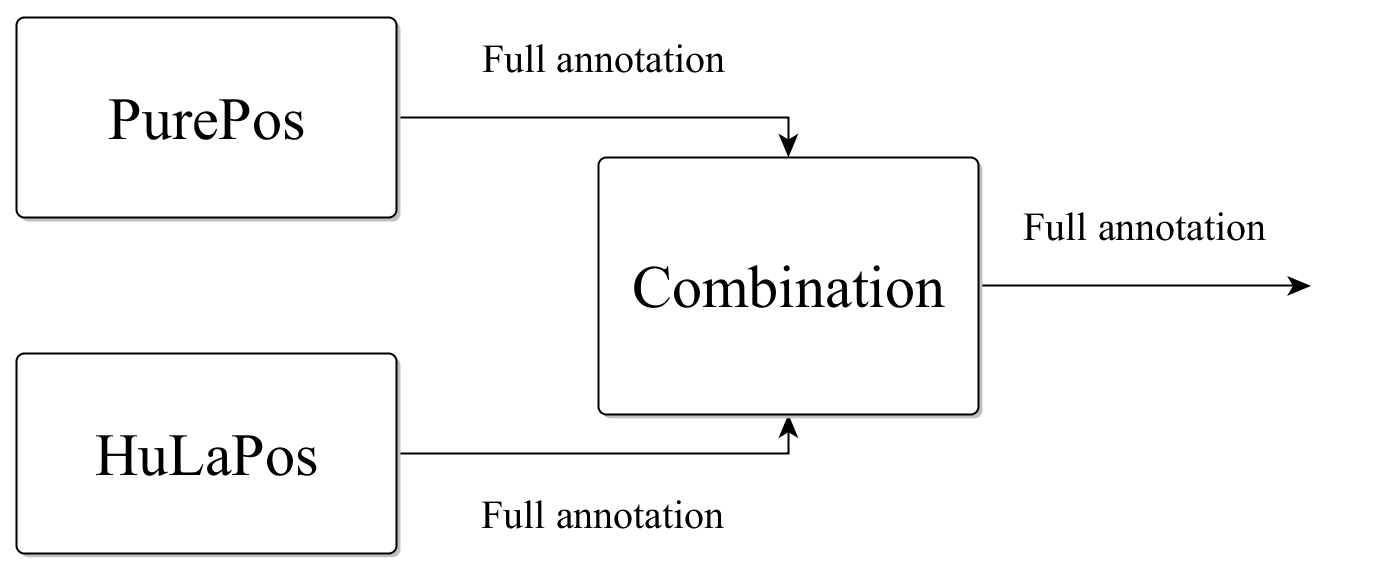
\includegraphics[scale=0.2]{MorphTagging/comb1.png} 
  \caption{Combining the output of two morphological taggers}
  \label{fig:comb1}
\end{figure}

\subsubsection{Combining PoS taggers only}

Another plausible scheme is to combine only the \acrshort{pos} tagger modules of the tools (see Figure \ref{fig:comb2}).
However, in doing so, one has to deal with lemmatization as well.
A straightforward solution for this to employ the lemmatizer of the better annotator tool (PurePos).
Following this, the best tag selection model could be constructed (cf.
Table \ref{tab:comb-reduction-rates}) using IB learning with FS4 features.

\begin{figure}[H]
  \centering
  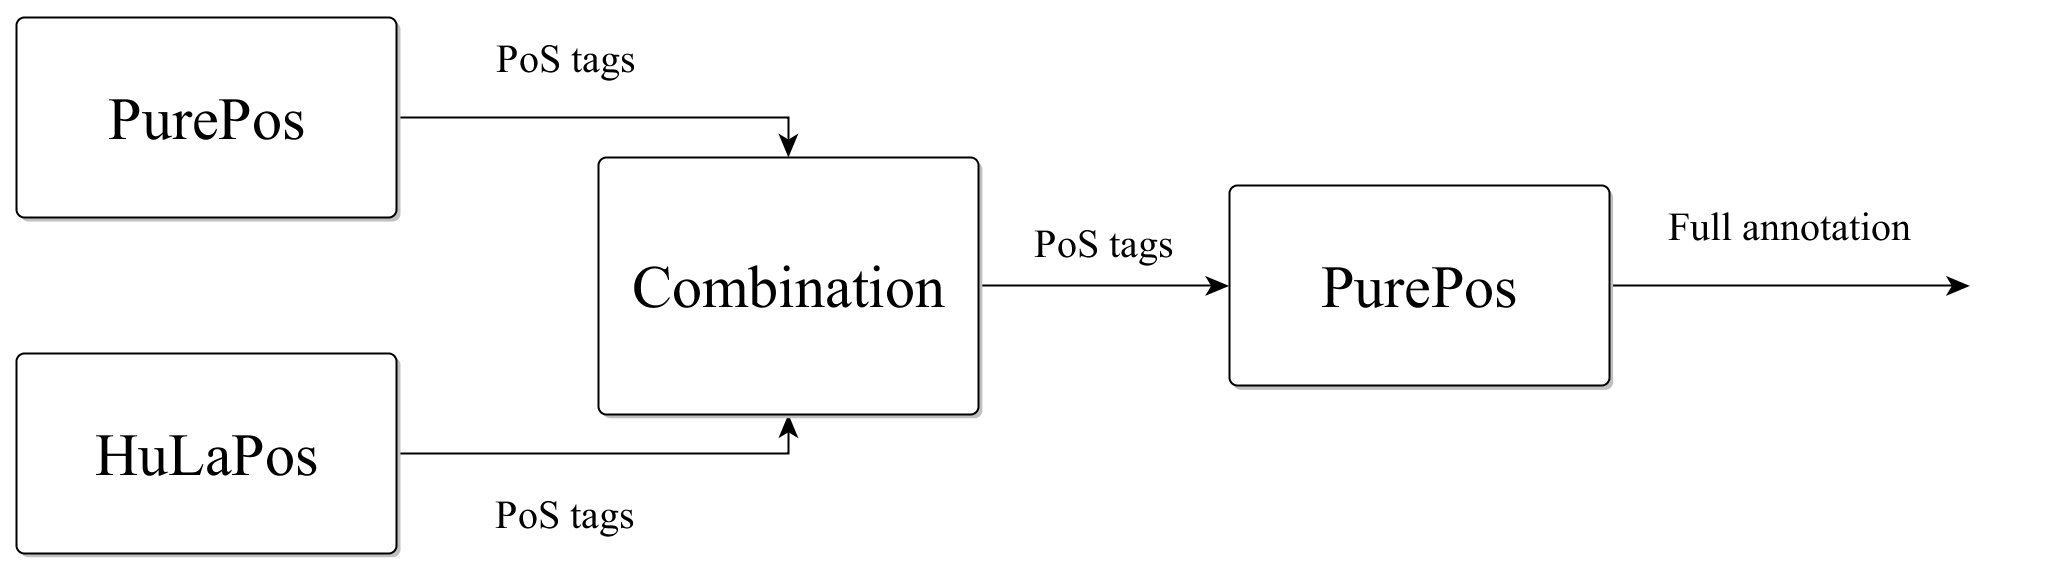
\includegraphics[scale=0.2]{MorphTagging/comb2.png} 
  \caption{Combining the output of two PoS taggers and using also a lemmatizer}
  \label{fig:comb2}
\end{figure}

Although this algorithm allows us to create a better morpho-syntactic tagger compared to that of above, the gain in lemmatization remains much lower (6.81\%).
Consequently, the overall accuracy improvement measured in the development set (25.26\%) is inferior.

\subsubsection{Multiple metalearners}

Finally, the best results are produced using two level-1 learners: one of them chooses the better lemmatizer while the other selects the optimal \acrshort{pos} tagger (cf. Figure \ref{fig:comb3}).
In that  way, this architecture can incorporate the best lemma and tag candidates (as in Table \ref{tab:comb-reduction-rates}) yielding superior performance.
However, a drawback of this configuration that it may result in incompatible tag-lemma pairs\footnote{A lemma and a tag for a word is incompatible if the \acrshort{ma} can analyze the word, but no analysis contains both the lemma and the morpho-syntactic label.}.
To overcome this problem, this combination scheme is enhanced with the Humor morphological analyzer.
This component is used to discover and fix incompatibilities.
With this enhancement, we achieved  32.42\% of improvement on the development set.

\begin{figure}[H]
  \centering
  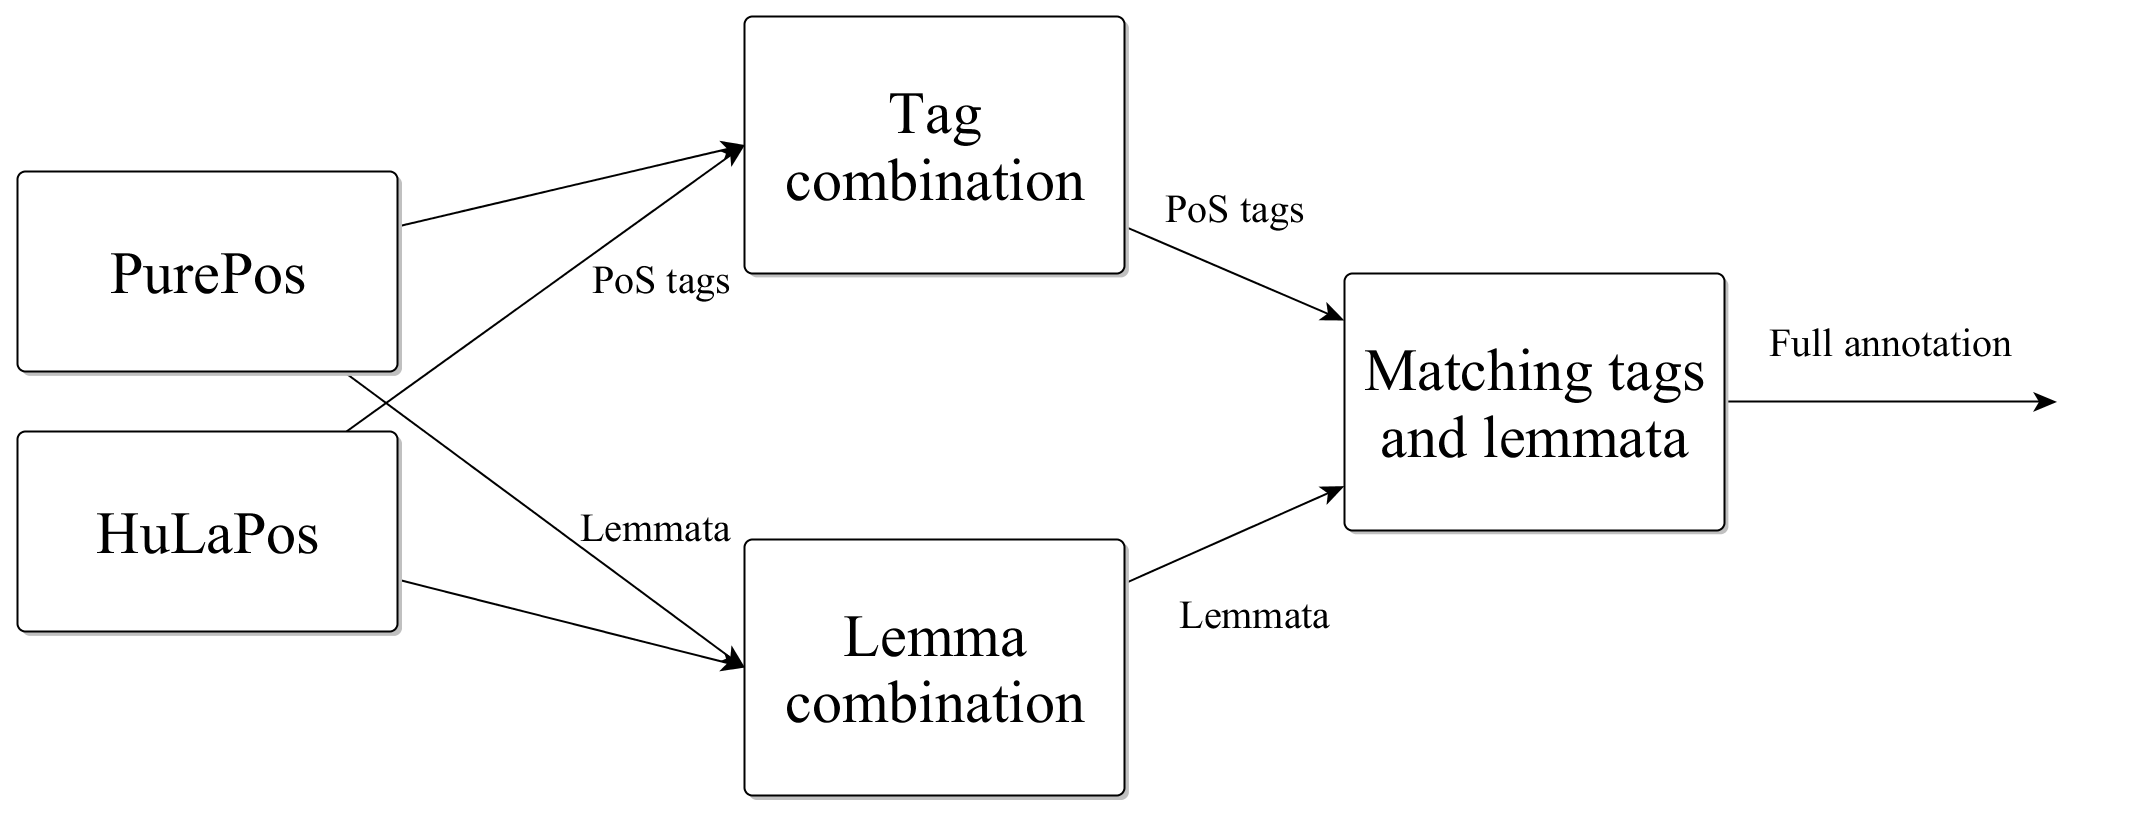
\includegraphics[scale=0.2]{MorphTagging/comb3.png} 
  \caption{Combining the output of two PoS taggers and lemmatizers}
  \label{fig:comb3}
\end{figure}

\subsection{Evaluation}

%In order to validate our hypothesis, stating that the last configuration performs the best, improvements
%Combination schemes presented are evaluated on the unseen test set. %, confirming the results presented above.

\begin{table}[H]
\centering
\caption{Relative error rate reduction on the test set compared to PurePos}\label{tab:comb-eval}
\begin{tabular}{l r r r}
\hline
System & Tagging & Lemmatization & Full disamb. \\
\hline
\textit{Oracle} & 48.60\% & 59.42\% & 51.53\% \\
Disamb. combination & 23.23\% & 23.55\% & 26.86\% \\
Tagger combination & 22.76\% & 13.77\% & 23.81\% \\
Multiple metalearners & 25.07\% & 29.89\% & \underline{28.90\%} \\
\hline
\end{tabular}
\end{table}

All the presented combination schemes are evaluated on the unseen test set. %, confirming the results presented above.
Results show (cf. Table \ref{tab:comb-eval}) that the hybrid architecture using a morphological analyzer achieved the best performance.
While other schemes could also increase the accuracy of PurePos, it resulted in the best tagging precision (98.90\%) of fixing 28.90\% of the baseline system's errors.
This improvement score also shows that our system could capture more then half of the cases which can be fixed by a hypothetical oracle combinator.
Further on, the proposed method also gives the highest error rate reduction in both \acrshort{pos} tagging and lemmatization.
Concerning statistical significance, both the improvements of the presented schemes and their differences are significant at p < 0.05 (using Wilcoxon test of paired samples).
These results show that our new combination architecture can be used in cases when very high disambiguation accuracy is crucial.
Finally, we also confirmed that PurePos and HuLaPos complement each other well resulting in an improved morphological tagger. 



 

 

 

 


 
